    % =============================================================================
% RESULTADOS
%
% Fontes dos números: docs/ANALISE-RODADA-{1..6}.md, docs/SONDA-MOTORES.md,
% docs/MAPA-TCC-O-QUE-REESCREVER.md e docs/auditoria-q4/ no repositório da
% pipeline. O plano de redação está em docs/PLANO-ESCRITA-RESULTADOS.md.
%
% A rodada comercial (gpt-6-luna, 2026-09-30) foi incorporada em tab:modelos,
% no fim de sec:modelos, em fig:recall-comparado, no item "Escopo de modelos"
% das limitações e em subsec:supressao. Fonte: docs/ANALISE-RODADA-COMERCIAL.md.
% A extensão com raciocínio (gpt-6-luna@low/@high, 2026-10-01) entrou no fim de
% sec:modelos (tab:raciocinio), em fig:recall-comparado, nas limitações, em
% subsec:supressao e em subsec:consequencias. Fonte: o mesmo documento, §8.
% =============================================================================

\chapter{Resultados}
\label{cap:resultados}

Este capítulo apresenta os resultados do experimento descrito no Capítulo~\ref{cap:metodologia}. A exposição segue as cinco perguntas declaradas na Seção~\ref{sec:metricas} (a Questão Geral e as questões Q1 a Q4) e dedica uma seção às causas do teto de detecção da camada simbólica (Seção~\ref{sec:eliminacao}), porque esse teto é o fator que mais limita os demais resultados, e a investigação das suas causas é um resultado por si só.

Duas leituras atravessam o capítulo e convém antecipá-las. A primeira é que a arquitetura cumpre o que foi projetada para cumprir: como filtro de alertas, ela remove a maior parte do ruído produzido pelo analisador estático, de forma replicada em populações distintas com o modelo principal, o \texttt{qwen2.5-coder:7b}, embora o ganho do \textit{prompt} especialista nesse papel não se repita no segundo modelo local, o \texttt{gemma2:9b}, nem no comercial, o \texttt{gpt-6-luna}. A segunda é que ela não cumpre o que a literatura frequentemente lhe atribui: o componente neural não recupera as vulnerabilidades que o componente simbólico deixa passar. As duas afirmações convivem, e distingui-las exige olhar separadamente os dois modos de execução descritos na Seção~\ref{subsec:modos}.

Os resultados vêm de uma sequência de rodadas, cada uma uma execução completa sobre a população, resumidas na Tabela~\ref{tab:rodadas}. Nas Rodadas 1 a 6, cada rodada muda uma única variável em relação à anterior, de modo que qualquer diferença entre duas rodadas seguidas pode ser atribuída a essa variável. A Rodada 3, a primeira sobre a população completa de 2.328 casos, é a referência do modo de filtro. A sétima rodada completa a comparação entre os dois modelos locais e testa outra forma de orientar o \textit{prompt} especialista, e a rodada comercial verifica até onde as conclusões se estendem a um modelo comercial, com e sem raciocínio (Seção~\ref{sec:modelos}).

Dois esclarecimentos valem para o capítulo inteiro. O primeiro é que, na sétima rodada, as fichas do \textit{prompt} especialista (Seção~\ref{sec:prompts}) foram escritas por regra do Semgrep, e não por CWE, como nas demais. O segundo é que as Rodadas 4 a 6 foram executadas uma segunda vez, com a mesma configuração, para permitir a comparação caso a caso com as rodadas posteriores. Os números citados são os da primeira execução, e a segunda indica quais deles se repetem (Seção~\ref{sec:limitacoesresultados}).

\begin{table}[htpb]
    \centering
    \caption[As rodadas do experimento]{As rodadas do experimento. B: \textit{prompt} \textit{baseline}; E: \textit{prompt} especialista; ``diretos'': as versões dos dois \textit{prompts} que perguntam sobre o código, e não sobre o alerta (Seção~\ref{subsec:enquadramento})}
    \label{tab:rodadas}
    \renewcommand{\arraystretch}{1.3}
    \setlength{\tabcolsep}{3pt}
    \footnotesize
    \begin{tabular}{|p{1.7cm}|p{3.0cm}|p{1.4cm}|p{1.9cm}|p{4.6cm}|p{1.5cm}|}
        \hline
        \textbf{Rodada} & \textbf{Modelo} & \textbf{Modo} & \textbf{\textit{Prompts}} & \textbf{O que muda} & \textbf{Seções} \\
        \hline
        1 & \texttt{qwen2.5-coder:7b} & filtro & B, E & Primeira execução, sobre 948 casos & \ref{sec:geral} \\
        \hline
        2 & \texttt{qwen2.5-coder:7b} & filtro & B, E & Critério estrito: o alerta só conta como detecção se a regra declarar exatamente a CWE do caso & \ref{sec:geral}, \ref{subsec:q1pareado} \\
        \hline
        3 & \texttt{qwen2.5-coder:7b} & filtro & B, E & População completa, de 2.328 casos; referência do modo de filtro & \ref{sec:geral} a \ref{sec:q4} \\
        \hline
        4 & \texttt{qwen2.5-coder:7b} & triagem & B, E & Primeira execução do modo de triagem, com o contexto reduzido ao código & \ref{subsec:q1controle}, \ref{subsec:q2distancia} \\
        \hline
        5 & \texttt{qwen2.5-coder:7b} & triagem & B, E diretos & Pergunta sobre o código, e não sobre o alerta & \ref{subsec:q1enquadramento}, \ref{subsec:q2triagem} \\
        \hline
        6 & \texttt{gemma2:9b} & triagem & B, E diretos & Troca do modelo & \ref{subsec:q2triagem}, \ref{sec:modelos} \\
        \hline
        7 & \texttt{qwen2.5-coder:7b} e \texttt{gemma2:9b} & filtro e triagem & B, E no filtro; E direto na triagem & Testa fichas por regra do Semgrep, em vez de por CWE; e executa o \texttt{gemma2:9b} no modo de filtro, com os dois \textit{prompts} & \ref{subsec:q1pareado}, \ref{subsec:q1fichas}, \ref{sec:modelos} \\
        \hline
        Comercial & \texttt{gpt-6-luna}, sem raciocínio & filtro e triagem & B, E e diretos & Modelo comercial; cada modo executado duas vezes, por não haver semente fixa & \ref{sec:modelos} \\
        \hline
        Comercial com raciocínio & \texttt{gpt-6-luna}, esforço baixo e alto & filtro e triagem & B, E e diretos & Raciocínio do modelo ligado & \ref{sec:modelos} \\
        \hline
        Segunda execução & mesmos das Rodadas 4 a 6 & triagem & os mesmos & Mesma configuração, para comparação caso a caso com as rodadas posteriores & \ref{sec:limitacoesresultados} \\
        \hline
    \end{tabular}
    \fontepesquisa
\end{table}

% =============================================================================
\section{O Ponto de Partida: o que Chega ao Modelo}
\label{sec:partida}

A Questão Q2 tem duas metades: pergunta se a arquitetura reduz o volume de falsos positivos \textit{e} se o faz sem introduzir falsos negativos. No modo de filtro, a segunda metade não é respondível. O motivo é visível na Figura~\ref{fig:funil}, que acompanha os 2.328 casos da população até o modelo de linguagem: dos 797 casos de gabarito vulnerável, o Semgrep emitiu alerta na CWE do caso sobre 19, e apenas esses chegam ao modelo. É um número irrisório: com 19 casos, cada acerto ou erro do modelo move o \textit{recall} em mais de cinco pontos percentuais, o que não basta para medir falsos negativos com alguma confiança. E o número não crescia com mais coleta, como mostra a Seção~\ref{sec:eliminacao}.

\begin{figure}[htpb]
    \centering
    \caption[O funil da população até o modelo de linguagem]{O caminho dos 2.328 casos da população até o modelo de linguagem, no modo de filtro (Rodada 3). As larguras são proporcionais às contagens}
    \label{fig:funil}
    \resizebox{\textwidth}{!}{
    \begin{tikzpicture}[
        font=\small,
        rot/.style={anchor=east, font=\small\bfseries, align=right, text width=30mm},
        cnt/.style={font=\footnotesize, align=center}
    ]
        % escala: 12 cm = 2.328 casos (1 caso = 0,0051546 cm)
        \node[rot] at (-0.3,0.3) {População};
        \fill[black!15] (0,0) rectangle (12,0.6);
        \node[cnt] at (6,0.3) {2.328 casos};

        \node[rot] at (-0.3,-1.2) {Gabarito};
        \fill[green!20] (0,-1.5) rectangle (7.892,-0.9);
        \fill[red!20] (7.892,-1.5) rectangle (12,-0.9);
        \node[cnt] at (3.946,-1.2) {1.531 seguros};
        \node[cnt] at (9.946,-1.2) {797 vulneráveis};

        \node[rot] at (-0.3,-2.7) {Semgrep\\\footnotesize(Fase 1)};
        \fill[orange!35] (0,-3.0) rectangle (4.165,-2.4);
        \fill[black!6] (4.165,-3.0) rectangle (7.892,-2.4);
        \fill[blue!70] (7.892,-3.0) rectangle (7.990,-2.4);
        \fill[black!6] (7.990,-3.0) rectangle (12,-2.4);
        \draw[black!40] (4.165,-3.0) -- (4.165,-2.4);
        \node[cnt] at (2.083,-2.7) {808 com alerta (ruído)};
        \node[cnt] at (6.029,-2.7) {723 sem alerta};
        \node[cnt] at (10.0,-2.7) {778 não detectados};

        \node[rot] at (-0.3,-4.2) {LLM\\\footnotesize(modo de filtro)};
        \fill[orange!35] (0,-4.5) rectangle (4.165,-3.9);
        \draw[dashed, black!30] (4.165,-4.5) rectangle (7.892,-3.9);
        \draw[dashed, black!30] (7.990,-4.5) rectangle (12,-3.9);
        \fill[blue!70] (7.892,-4.5) rectangle (7.990,-3.9);
        \node[cnt] at (2.083,-4.2) {808 alarmes falsos};
        \node[cnt, text=black!55] at (6.029,-4.2) {723 fora do modelo};
        \node[cnt, text=black!55] at (10.0,-4.2) {778 fora do modelo};
        \node[cnt, anchor=west] (d19) at (8.4,-5.0) {19 vulneráveis detectados};
        \draw[-{Latex[length=1.8mm]}] (d19.west) -- (7.99,-4.5);

        \draw[dashed, black!40] (0,-2.4) -- (0,-1.5) (4.165,-3.9) -- (4.165,-3.0)
              (7.892,-3.9) -- (7.892,-1.5) (7.990,-3.9) -- (7.990,-3.0) (12,-2.4) -- (12,-1.5);
    \end{tikzpicture}
    }
    \fontepesquisa
\end{figure}

A Figura~\ref{fig:funil} se lê de cima para baixo, uma linha por etapa. A primeira linha é a população inteira, e a segunda a divide pelo gabarito em 1.531 casos seguros e 797 vulneráveis. A terceira mostra o que o Semgrep fez com cada lado. Entre os seguros, 808 produziram alerta, pouco mais da metade, e esses alarmes falsos são o ruído que a triagem neural deve filtrar. Os outros 723 não produziram alerta e já estão resolvidos sem o modelo. Entre os vulneráveis, o Semgrep emitiu alerta na CWE rotulada sobre apenas 19, a faixa azul estreita, o que dá uma taxa de detecção de 2,38\% sobre a classe positiva inteira. Os 778 restantes são o ponto cego do analisador. A última linha mostra o que chega ao modelo no modo de filtro: apenas os casos com alerta. Os 723 seguros sem alerta e os 778 vulneráveis não detectados ficam de fora, e o modelo avalia 827 casos, dos quais 19 vulneráveis, uma taxa-base de positivos de 2,3\%. Esses 827 casos, sobre os quais o Semgrep emitiu alerta, formam a \textbf{pilha de alertas}: é o que um desenvolvedor receberia para revisar, e é sobre ela que o modelo atua no modo de filtro. A figura resume o problema do trabalho inteiro: o modelo recebe muito ruído para filtrar e quase nenhum caso vulnerável para confirmar.

Por isso as execuções também usam o modo de triagem (Seção~\ref{subsec:modos}), em que os 778 vulneráveis não detectados chegam ao modelo pela localização declarada no gabarito. Com eles, o modelo passa a avaliar todos os 797 casos vulneráveis, e não só 19. Como continua avaliando também os 808 alarmes falsos, a proporção de vulneráveis entre os casos que ele avalia, a taxa-base, sobe de 2,3\% para cerca de 50\%. Como nesse modo os campos do alerta são retirados de todos os casos, o modelo recebe ali menos informação do que no modo de filtro, o que acabou se revelando um achado por si só (Seção~\ref{subsec:q1controle}).

Uma dúvida possível é se os casos vindos do gabarito, por virem de outra fonte, ficariam mais fáceis de acertar. Não ficaram: na Rodada 4, o modelo acertou menos de 1\% deles, por razões discutidas na Seção~\ref{subsec:q1enquadramento}, enquanto nos 19 casos detectados pelo Semgrep, que servem de comparação (Seção~\ref{subsec:modos}), acertou entre 0\% e 15,8\%, conforme o \textit{prompt}. Como são só 19 casos, essa comparação é um indício, e não uma prova.

% =============================================================================
\section{Questão Geral: Redução da Fadiga de Alertas}
\label{sec:geral}

A Questão Geral pergunta como auxiliar o desenvolvedor na avaliação do resultado da análise estática de forma a reduzir a fadiga de alertas, e a metodologia associa a ela duas métricas: a Taxa de Redução de Alertas (TRA) e a Proporção de Falsos Positivos Filtrados. Ambas são medidas no modo de filtro, sobre os 827 alertas que chegam ao modelo: os 808 alarmes falsos e os 19 vulneráveis da Figura~\ref{fig:funil}. A TRA é calculada sobre todos eles, e a proporção de falsos positivos filtrados, apenas sobre os 808 alarmes falsos.

\begin{table}[htpb]
    \centering
    \caption[Métricas da Questão Geral]{Métricas da Questão Geral no modo de filtro (Rodada 3, \texttt{qwen2.5-coder:7b})}
    \label{tab:geral}
    \renewcommand{\arraystretch}{1.4}
    \begin{tabular}{|l|c|c|c|c|}
        \hline
         & \textbf{Alertas com} & & & \textbf{Alarmes falsos} \\
        \textbf{\textit{Prompt}} & \textbf{veredito} & \textbf{Descartados} & \textbf{TRA} & \textbf{descartados} \\
        \hline
        \textit{Baseline} & 825$^{*}$ & 701 & 85,0\% & 690 de 806$^{*}$ (85,6\%) \\
        \hline
        Especialista & 827 & 812 & 98,2\% & 796 de 808 (98,5\%) \\
        \hline
    \end{tabular}
    \par\vspace{2pt}{\footnotesize $^{*}$ Dois alarmes falsos ficaram sem veredito do \textit{baseline}, porque o modelo entrou em laço de geração, falha que se repetiu em todas as execuções.\par}
    \fontepesquisa
\end{table}

A Tabela~\ref{tab:geral} traz os valores. Com o \textit{prompt} especialista, o modelo descartou 812 dos 827 alertas, e a pilha que restaria para revisão humana cairia de 827 para 15. Dos 808 alarmes falsos, o especialista descartou 796, e o \textit{baseline}, 690 dos 806 que avaliou.

O valor mais relevante não é o de uma rodada, e sim a sua estabilidade. A TRA do \textit{prompt} especialista foi de 98,51\% na Rodada 1, 98,74\% na Rodada 2 e 98,19\% na Rodada 3, a última sobre uma população 146\% maior que as anteriores. Na Rodada 4, sobre a mesma pilha de alertas mas com o contexto reduzido ao código, foi de 98,31\%. A redução de ruído atravessa, portanto, três populações e duas formas de montar o contexto sem se mover mais de 0,6 ponto percentual. É o resultado mais robusto do experimento com o \texttt{qwen2.5-coder:7b}, e ele é específico desse modelo: executado no mesmo modo de filtro, sobre os mesmos casos, o \texttt{gemma2:9b} descartou 78,5\% dos alertas com o \textit{prompt} especialista, menos do que com o seu próprio \textit{baseline} (83,9\%), resultado discutido na Seção~\ref{subsec:q1pareado}, e o modelo comercial, \texttt{gpt-6-luna}, descartou de 66\% a 70\%, com qualquer dos dois \textit{prompts} e com ou sem raciocínio (Seção~\ref{sec:modelos}).

A TRA, contudo, não pode ser lida sozinha. Ela é definida como a fração de alertas que o modelo descarta, de modo que um classificador que descartasse todos os alertas alcançaria o valor máximo. A TRA de 98,2\% vem acompanhada de uma taxa de falsos negativos de 84,2\% sobre os 19 casos vulneráveis, e esse par caracteriza uma estratégia de supressão agressiva, discutida na Seção~\ref{subsec:supressao}. A resposta à Questão Geral é, assim, que a arquitetura auxilia o desenvolvedor usando o modelo de linguagem como filtro depois do analisador: com o modelo principal e o \textit{prompt} especialista, os alertas a revisar caem de 827 para 15. Esse auxílio, porém, tem um custo, detalhado na Q2: 16 dos 19 alertas verdadeiros seriam descartados pelo modelo junto com o ruído e nem chegariam à revisão.

% =============================================================================
\section{Q1: Impacto do Enriquecimento Semântico na Precisão}
\label{sec:q1}

A Q1 pergunta pelo impacto do enriquecimento semântico na precisão do modelo, e a metodologia associa a ela Precisão, \textit{F1-Score} e MCC. A comparação é pareada por construção: os dois \textit{prompts} avaliam exatamente os mesmos casos, sob o mesmo modelo, a mesma semente e temperatura zero. As três métricas declaradas dependem da célula de verdadeiros positivos e, no modo de filtro, repousam sobre 19 casos vulneráveis. Por isso, a comparação principal da Q1 é feita pelo teste de McNemar, que usa todos os casos pareados.

\subsection{Comparação Pareada entre os Tipos de \textit{Prompt}}
\label{subsec:q1pareado}

A comparação entre os dois \textit{prompts} é feita sobre os mesmos 825 alertas, contando em quais casos cada um acerta. A Tabela~\ref{tab:mcnemar} apresenta essa contagem para a Rodada 3. A informação relevante está nas duas células em que os \textit{prompts} discordam.

\begin{table}[htpb]
    \centering
    \caption[Discordâncias entre os \textit{prompts} (McNemar)]{Tabela de discordâncias entre os \textit{prompts} \textit{baseline} e especialista (Rodada 3, 825 casos pareados)}
    \label{tab:mcnemar}
    \renewcommand{\arraystretch}{1.4}
    \begin{tabular}{|l|c|c|}
        \hline
         & \textbf{Especialista acerta} & \textbf{Especialista erra} \\
        \hline
        \textbf{\textit{Baseline} acerta} & 693 & 5 \\
        \hline
        \textbf{\textit{Baseline} erra} & 104 & 23 \\
        \hline
    \end{tabular}
    \fontepesquisa
\end{table}

Em 104 casos apenas o especialista acerta, contra 5 em que apenas o \textit{baseline} acerta, diferença estatisticamente significativa (McNemar, $\chi^2 = 88{,}11$, $p < 0{,}0001$; Seção~\ref{sec:metricas}) e já observada na Rodada 2, com 100 contra 0. A vantagem concentra-se nos alarmes falsos: o especialista mantém 12, contra 116 do \textit{baseline}. Nos 19 vulneráveis, ao contrário, acerta menos (3 contra 8). As métricas associadas à Q1 pela metodologia apontam na mesma direção (a precisão passa de 6,5\% para 20\%, o \textit{F1} de 0,11 para 0,18 e o MCC de $+0{,}12$ para $+0{,}16$), mas dependem desses 19 casos e, por isso, são menos confiáveis que o teste pareado.

No segundo modelo local, a vantagem \textbf{se inverte}. Com o \texttt{gemma2:9b}, nas mesmas condições, em 96 casos apenas o \textit{baseline} acerta, contra 49 em que apenas o especialista acerta ($p = 0{,}0001$), e os alarmes falsos sobem de 127 para 173. O aumento concentra-se na CWE-327: a ficha dessa categoria descreve \textit{hash} fraco aplicado a senha, enquanto os alertas apontam configuração de TLS sem versão mínima, e o modelo combina os dois perigos. Nessa categoria, o especialista produziu 57 alarmes falsos em 93 alertas, contra 10 do \textit{baseline} (Seção~\ref{subsec:q1fichas}).

No modelo comercial, o \texttt{gpt-6-luna}, executado duas vezes, a vantagem não se confirma: a diferença entre os \textit{prompts} é significativa em uma execução ($p = 0{,}032$) e não na outra ($p = 0{,}227$), e o excesso de alarmes do especialista concentra-se na mesma CWE-327 (Seção~\ref{sec:modelos}). No modo de filtro, portanto, o efeito depende do modelo: o enriquecimento semântico reduz os falsos positivos com o \texttt{qwen2.5-coder:7b}, aumenta-os com o \texttt{gemma2:9b} e não produz diferença estável com o modelo comercial. No modo de triagem, por outro lado, o especialista supera o \textit{baseline} nas duas execuções desse modelo.

\subsection{O \textit{Baseline} como Controle: uma Correção}
\label{subsec:q1controle}

O grupo de controle do modo de triagem permitiu um experimento que nenhuma rodada anterior permitia. Os 19 casos vulneráveis detectados pelo Semgrep foram avaliados na Rodada 3, no modo de filtro, e na Rodada 4, no modo de triagem, com os mesmos identificadores, o mesmo modelo, os mesmos \textit{templates} de \textit{prompt}, a mesma semente e temperatura zero. A única variável entre as duas execuções é o contexto: com os campos do alerta, na Rodada 3; só com o código, na Rodada 4. O \textit{prompt} especialista acertou 3 dos 19 nas duas rodadas. O \textit{baseline} acertou 8 na Rodada 3 e \textbf{zero} na Rodada 4: os oito verdadeiros positivos foram a zero, e nenhum caso foi ganho.

A explicação é direta. O \textit{prompt} \textit{baseline} não recebe CWE, definição nem heurística: por desenho, é a condição de controle. Mas, no modo de filtro, o contexto hidratado abre com o identificador da regra e a mensagem do Semgrep, e essa mensagem nomeia a fraqueza (Figura~\ref{fig:contexto-braco}). O \textit{baseline} utilizado nas Rodadas 1 a 3 não era, portanto, um controle limpo: parte do seu desempenho provinha de ler a resposta no próprio enunciado. O especialista não se move porque o sinal dele vem da ficha da CWE, que continua presente nos dois modos.

A consequência para a Q1 é que a diferença medida entre os dois \textit{prompts} nas Rodadas 1 a 3 \textbf{subestima} o efeito do enriquecimento semântico, porque o \textit{baseline} já se encontrava parcialmente enriquecido pelo metadado da regra. A correção não é feita em silêncio sobre os números da Tabela~\ref{tab:mcnemar}: eles continuam válidos como medida do que os dois \textit{prompts} fazem no sistema implantável, em que a mensagem do motor está presente, mas não como medida isolada da engenharia de \textit{prompt}. Pelo mesmo motivo, o \textit{baseline} do modo de triagem não é comparável ao \textit{baseline} do modo de filtro: não é o mesmo componente sobre mais casos, e sim um tratamento mais pobre. O especialista não sofre dessa distinção, e é o único cuja série atravessa os dois modos com o mesmo significado.

\subsection{O Enquadramento do \textit{Prompt} como Variável}
\label{subsec:q1enquadramento}

No modo de triagem, os \textit{prompts} originais perguntam se o alerta é verdadeiro ou falso positivo, pergunta que não faz sentido para os 778 casos vindos do gabarito, que não têm alerta (Seção~\ref{subsec:enquadramento}). Para esses casos, responder ``falso positivo'' pode ser apenas coerente com a pergunta feita, e não uma falha de detecção. A Rodada 5 isolou essa variável: manteve modelo, população e semente e trocou apenas a pergunta, adotando as versões diretas dos dois \textit{prompts}, que perguntam se o código contém a fraqueza. A informação entregue ao modelo é a mesma: muda só a pergunta.

A troca teve efeito. O \textit{recall} do especialista no modo de triagem subiu de 1,3\% para 5,1\%, e o ganho foi maior justamente nos casos sem alerta: neles, o acerto quase quintuplicou (de 0,92\% para 4,47\%), enquanto nos 19 casos vindos de alerta dobrou (de 15,8\% para 31,6\%). A diferença entre os dois \textit{prompts}, ausente na Rodada 4 (14 contra 12 casos discordantes, $p = 0{,}84$), passou a favorecer o especialista na Rodada 5 (63 contra 36, $p = 0{,}009$).

Na segunda execução da Rodada 5, apenas parte desses números se repete. O \textit{recall} do especialista nos casos sem alerta se mantém (4,49\% contra 4,47\%), mas o acerto nos 19 casos com alerta cai para 4 (21,1\%), e a vantagem do especialista deixa de ser significativa (58 contra 40, $p = 0{,}086$). A leitura que se sustenta é, portanto, mais modesta: a pergunta direta aumenta de forma reprodutível o \textit{recall} nos casos sem alerta, e há apenas \textbf{indicação} de vantagem do especialista nesse enquadramento. O fato de poucos casos bastarem para desfazer a significância mostra quão frágeis são as diferenças medidas sobre 19 casos.

Ainda assim, o ganho é pequeno e não resolve o problema. Dos 54 vereditos ``vulnerável'' que o especialista passou a emitir, 30 estavam certos e 24 errados, pouco melhor que o acaso, já que metade dos casos do modo de triagem é vulnerável. Sem a CWE, o \textit{baseline} direto piora: dos seus 37 novos vereditos ``vulnerável'', apenas 7 estavam certos, e o MCC vai a $-0{,}083$, abaixo do acaso. Conclui-se que a forma da pergunta é, ela própria, uma variável que afeta o \textit{recall}, e que a Rodada 4 mediu o modo de triagem com uma pergunta que não se aplicava a metade dos casos. Por isso, deste ponto em diante, os números do modo de triagem citados neste capítulo são os da pergunta direta.

\subsection{Fichas por CWE ou por Regra}
\label{subsec:q1fichas}

As fichas que alimentam o \textit{prompt} especialista foram escritas por CWE, antes da primeira execução, a partir da definição da fraqueza e da documentação da biblioteca padrão de Go, sem consulta às amostras nem às regras do Semgrep (Seção~\ref{sec:prompts}). Por isso, elas não descrevem a regra que emite cada alerta, e em algumas categorias a construção apontada pela regra difere da exemplificada na ficha. Na CWE-327, por exemplo, a ficha trata de \textit{hash} fraco aplicado a senha, e os 93 alertas da população são de configuração de TLS sem versão mínima. Com o \texttt{qwen2.5-coder:7b}, essa diferença não aparece nos números, porque nessas categorias os dois \textit{prompts} acertam o mesmo (91 de 93 alertas na CWE-327, 93 de 94 na CWE-94 e 75 de 75 na CWE-665). Com o \texttt{gemma2:9b}, ela aparece, e é na CWE-327 que se concentram os alarmes falsos acrescentados pelo seu especialista (Seção~\ref{subsec:q1pareado}).

A sétima rodada testou a alternativa, uma ficha para cada regra do Semgrep que dispara, nos dois modelos locais e nos dois modos, comparando caso a caso com as fichas por CWE. Nos quatro cenários, o \textit{recall} é praticamente o mesmo, e a diferença está nos alarmes falsos. As fichas por CWE tiveram menos alarmes falsos em três deles. No modo de triagem, foram 39 contra 119 com o \texttt{qwen2.5-coder:7b} (em 80 casos só as fichas por CWE acertam, contra 2 em que só as fichas por regra acertam, $p < 0{,}0001$) e 104 contra 210 com o \texttt{gemma2:9b} (116 contra 12, $p < 0{,}0001$). No modo de filtro do \texttt{qwen2.5-coder:7b}, foram 12 contra 20, com os mesmos 3 dos 19 vulneráveis reconhecidos, mas essa diferença depende de poucos casos e não é significativa (12 contra 4, $p = 0{,}077$).

A exceção é o modo de filtro do \texttt{gemma2:9b}, em que as fichas por regra tiveram 69 alarmes falsos, contra 171 das fichas por CWE nos casos com veredito válido nas duas versões (19 contra 121, $p < 0{,}0001$). É justamente o caso em que a ficha por CWE descreve uma fraqueza diferente da apontada pelo alerta, e o modelo, que no modo de filtro vê a mensagem do alerta, mistura as duas. Os 57 alarmes falsos da CWE-327 desaparecem com a ficha por regra. As fichas por CWE tiveram, portanto, desempenho melhor em três dos quatro cenários, e são elas as usadas em todos os números deste capítulo.

Reunidas as quatro análises, a resposta à Q1 é que o enriquecimento semântico melhora a precisão do modelo, mas não de forma geral. No modo de filtro, ele reduz os falsos positivos com o \texttt{qwen2.5-coder:7b}, aumenta-os com o \texttt{gemma2:9b} e não produz diferença estável com o modelo comercial. Com o \texttt{qwen2.5-coder:7b}, esse efeito está subestimado nas Rodadas 1 a 3, porque o \textit{baseline} lia a fraqueza na mensagem do Semgrep (Seção~\ref{subsec:q1controle}). E a própria forma da pergunta altera o resultado, a ponto de o efeito no modo de triagem só poder ser medido com a pergunta direta. A forma de escrever as fichas também importa. As fichas por CWE tiveram menos alarmes falsos que as fichas por regra em três dos quatro cenários, e só perderam quando a ficha descrevia uma fraqueza diferente da apontada pelo alerta.

% =============================================================================
\section{Q2: Redução de Falsos Positivos sem Introduzir Falsos Negativos}
\label{sec:q2}

A Q2 tem duas metades, e elas se respondem em modos diferentes. A primeira, reduzir o volume de falsos positivos, é respondida no modo de filtro e coincide com a Questão Geral (Seção~\ref{sec:geral}). A segunda, sem introduzir falsos negativos, só pôde ser respondida com a classe positiva inteira, no modo de triagem. As métricas associadas pela metodologia são o \textit{Recall} e a Taxa de Falsos Negativos (TFN).

\subsection{No Modo de Filtro: o Sistema Implantável}
\label{subsec:q2filtro}

No modo de filtro, a segunda metade da Q2 se traduz numa pergunta direta: dos 19 vulneráveis que chegam ao modelo, quantos ele descarta junto com o ruído? A Tabela~\ref{tab:filtro} reúne o desempenho das configurações avaliadas sobre a pilha real de alertas. As quatro primeiras linhas são execuções do modo de filtro, com os dois modelos locais nas mesmas condições. As duas últimas vêm do modo de triagem, restritas aos casos vindos de alerta, e não são diretamente comparáveis às primeiras, porque ali o modelo não recebe os campos do alerta e a pergunta é sobre o código.

\begin{table}[htpb]
    \centering
    \caption[Desempenho na tarefa de filtro]{Desempenho na tarefa de filtro, sobre a pilha real de alertas (19 casos vulneráveis em 827, salvo indicação)}
    \label{tab:filtro}
    \renewcommand{\arraystretch}{1.4}
    \small
    \begin{tabular}{|l|c|c|c|c|c|c|}
        \hline
        \textbf{Modelo, \textit{prompt} (rodada)} & \textbf{VP} & \textbf{FN} & \textbf{FP} & \textbf{\textit{Recall}} & \textbf{TRA} & \textbf{MCC} \\
        \hline
        \multicolumn{7}{|l|}{\textit{Modo de filtro}} \\
        \hline
        \texttt{qwen2.5-coder:7b}, \textit{baseline} (R3) & 8 & 11 & 116 & 42,1\% & 85,0\% & $+0{,}116$ \\
        \hline
        \texttt{qwen2.5-coder:7b}, especialista (R3) & 3 & 16 & 12 & 15,8\% & 98,2\% & $+0{,}161$ \\
        \hline
        \texttt{gemma2:9b}, \textit{baseline} (R7)$^{*}$ & 5 & 14 & 127 & 26,3\% & 83,9\% & $+0{,}043$ \\
        \hline
        \texttt{gemma2:9b}, especialista (R7)$^{*}$ & 4 & 15 & 173 & 21,1\% & 78,5\% & $-0{,}002$ \\
        \hline
        \multicolumn{7}{|l|}{\textit{Pilha de alertas lida dentro do modo de triagem, enquadramento direto}$^{\dagger}$} \\
        \hline
        \texttt{qwen2.5-coder:7b}, especialista direto (R5) & 6 & 13 & 35 & 31,6\% & 95,0\% & $+0{,}188$ \\
        \hline
        \texttt{gemma2:9b}, especialista direto (R6)$^{\ddagger}$ & 7 & 11 & 107 & 38,9\% & 86,1\% & $+0{,}108$ \\
        \hline
    \end{tabular}
    \par\vspace{2pt}{\footnotesize $^{*}$ Sobre 822 vereditos válidos dos mesmos 827 casos, 19 deles vulneráveis. $^{\dagger}$ Não são execuções do modo de filtro: são os casos vindos de alerta avaliados no modo de triagem, em que o contexto não traz os campos do alerta e a pergunta é sobre o código. $^{\ddagger}$ Sobre 18 casos vulneráveis: a comparação pareada com a Rodada 5 exclui um caso sem veredito válido por estouro da janela de contexto.\par}
    \fontepesquisa
\end{table}

A TFN é o complemento do \textit{recall}: com o \texttt{qwen2.5-coder:7b}, 57,9\% no \textit{baseline} e 84,2\% no especialista; com o \texttt{gemma2:9b}, 73,7\% e 78,9\%. TRA e TFN precisam ser lidas juntas, porque as duas sobem quando o modelo descarta mais. Com o \texttt{qwen2.5-coder:7b}, o especialista descarta quase tudo: reduz o ruído e perde a maior parte das vulnerabilidades, enquanto o \textit{baseline} descarta menos e preserva mais. Com o \texttt{gemma2:9b}, o especialista é pior nas duas direções: acerta um vulnerável a menos e mantém 46 alarmes falsos a mais (Seção~\ref{subsec:q1pareado}). O especialista direto do \texttt{qwen2.5-coder:7b} fica no meio: dobra o \textit{recall} do especialista original, mas a pilha para revisão sobe de 15 para 41 alertas.

O MCC do \texttt{qwen2.5-coder:7b}, entre $+0{,}11$ e $+0{,}19$, indica discriminação modesta, mas positiva, para uma taxa-base de 2,3\%. Já o do \texttt{gemma2:9b} no modo de filtro, entre $-0{,}002$ e $+0{,}043$, indica praticamente nenhuma. Esses valores, porém, repousam sobre 19 casos vulneráveis, e poucos acertos a mais ou a menos os alteram bastante: o MCC do especialista direto do \texttt{qwen2.5-coder:7b}, por exemplo, cai de $+0{,}188$ para $+0{,}110$ na reexecução da Rodada 5, que acerta 4 dos 19 vulneráveis em vez de 6. As diferenças de \textit{recall} e MCC entre as linhas da tabela indicam, portanto, ordem de grandeza, e não sustentam teste estatístico. O que a tabela sustenta com segurança é o lado dos alarmes falsos, medido sobre 808 alertas. Ainda assim, a leitura da segunda metade da Q2 no modo de filtro é clara: em todas as configurações da tabela, mais da metade dos vulneráveis que chegam ao modelo é descartada junto com o ruído.

\subsection{No Modo de Triagem: o Teto do Componente Neural}
\label{subsec:q2triagem}

No modo de triagem, o modelo avalia também os 778 casos vulneráveis que o analisador não detectou, os casos vindos do gabarito (Seção~\ref{subsec:modos}), chamados daqui em diante de \textbf{injetados}, e a segunda metade da Q2 ganha uma base bem maior: em vez de 19 vulneráveis, são 797. A pergunta passa a ser quantos dos casos que o analisador perdeu o modelo consegue recuperar. Sobre os injetados, a única métrica que faz sentido é o \textit{recall}: como todos são vulneráveis, não há entre eles alarmes falsos nem verdadeiros negativos, e métricas como precisão e MCC não se aplicam. A Tabela~\ref{tab:triagem} traz o \textit{recall} dos dois modelos locais sobre esses casos, com as versões diretas dos dois \textit{prompts} (Seção~\ref{subsec:q1enquadramento}).

\begin{table}[htpb]
    \centering
    \caption[\textit{Recall} sobre os casos não detectados pelo analisador]{\textit{Recall} sobre os casos vulneráveis não detectados pelo analisador (modo de triagem, enquadramento direto)}
    \label{tab:triagem}
    \renewcommand{\arraystretch}{1.4}
    \begin{tabular}{|l|c|c|c|}
        \hline
        \textbf{Modelo} & \textbf{\textit{Prompt}} & \textbf{\textit{Recall}} & \textbf{TFN} \\
        \hline
        \texttt{qwen2.5-coder:7b} & especialista direto & 4,31\% & 95,69\% \\
        \hline
        \texttt{gemma2:9b} & especialista direto & 7,41\% & 92,59\% \\
        \hline
        \texttt{qwen2.5-coder:7b} & \textit{baseline} direto & 1,05\% & 98,95\% \\
        \hline
        \texttt{gemma2:9b} & \textit{baseline} direto & 24,21\% & 75,79\% \\
        \hline
    \end{tabular}
    \fontepesquisa
\end{table}

Com o \textit{prompt} especialista, os modelos locais recuperam entre 4\% e 7\% dos injetados. O valor de 24,21\% do \textit{baseline} do \texttt{gemma2:9b} não indica que esse modelo reconheça melhor as fraquezas, e sim viés de resposta: ele tende a responder ``vulnerável'' para quase tudo, tanto que a mesma configuração marca como vulneráveis 44\% dos alertas da pilha real, que é 97,8\% código seguro (Seção~\ref{sec:modelos}). Os valores se repetem na reexecução das Rodadas 5 e 6: 4,49\% e 6,52\% de \textit{recall} com o especialista; 1,19\% e 23,65\% com o \textit{baseline}. Em outras palavras, com o especialista, os dois modelos locais deixam passar mais de 92\% do que o analisador já havia perdido.

O modelo comercial, executado no mesmo modo e com a mesma pergunta, recupera mais. Sem raciocínio, chega a cerca de 17\% dos injetados, com os dois \textit{prompts}; com o raciocínio ligado, a 33\% e 39\% com o especialista, nos esforços baixo e alto, e a 41\% e 51\% com o \textit{baseline}, que nessa última configuração marca como vulneráveis 44\% dos alarmes falsos da pilha (Seção~\ref{sec:modelos}). Mesmo na configuração que mais recupera, metade dos casos que o analisador perde continua perdida.

A resposta à segunda metade da Q2 no modo de triagem é, portanto, a mesma nos três modelos: o componente neural não compensa o que o analisador deixa passar. Muda apenas a magnitude: TFN acima de 92\% nos modelos locais com o especialista, de cerca de 83\% no comercial sem raciocínio e de cerca de 50\% no comercial na configuração que mais alarma.

Esses números, além disso, são otimistas. No modo de triagem, o \textit{prompt} especialista recebe a CWE do gabarito, e o trecho de código entregue ao modelo é o apontado pelo gabarito: o modelo sabe qual fraqueza procurar e onde olhar, informação que, em produção, não existiria para um caso sem alerta. Mesmo com essa ajuda, os modelos locais recuperam de 4\% a 7\%. Há ainda uma pequena perda de vereditos, concentrada nas funções mais longas, discutida nas limitações do estudo (Seção~\ref{sec:limitacoesresultados}).

\subsection{A Distância entre os Modos}
\label{subsec:q2distancia}

A diferença entre os dois modos mede quanto se perde porque o modelo só julga o que o analisador emitiu, limitação do modo de filtro já apontada na metodologia (Seção~\ref{sec:limitacoes}). Para medi-la, usa-se o \textit{recall} sobre os 797 vulneráveis da população inteira, contando como perdido todo caso que o modelo não marcou como vulnerável, inclusive os que nunca chegaram a ele. Só assim os dois modos têm o mesmo denominador.

Como o modo de filtro só foi executado com os \textit{prompts} originais, a comparação direta usa esses \textit{prompts} nos dois modos (Rodadas 3 e 4). Nela, o especialista recupera 3 dos 797 vulneráveis no filtro (0,38\%) e 10 na triagem (1,25\%), uma diferença de só 0,88 ponto percentual. No \textit{baseline}, a diferença chega a ser negativa ($-0{,}63$ ponto), porque na triagem ele deixa de ver a mensagem do alerta, que no filtro lhe indicava a fraqueza (Seção~\ref{subsec:q1controle}).

Esse valor, porém, subestima a distância, porque a pergunta sobre o alerta não se aplica aos casos sem alerta (Seção~\ref{subsec:q1enquadramento}). Com a pergunta direta, o especialista chega a 5,1\% na triagem, e o filtro não poderia passar de 2,38\% (os 19 vulneráveis que chegam ao modelo, em 797): a distância é, portanto, de pelo menos 2,7 pontos. Mesmo vendo todos os casos, o modelo deixa passar mais de 94\% dos vulneráveis.

Restringir o modelo ao que o analisador emite tem, assim, um custo real, mas pequeno em valor absoluto, e nenhum dos dois modos sustenta a leitura de que bastaria deixar o modelo ver tudo. Essa distância, porém, mistura dois efeitos: quais casos chegam ao modelo e quanto contexto cada um traz, já que o modo de triagem entrega menos informação que o de filtro (Figura~\ref{fig:contexto-braco}). Atribuí-la inteira ao primeiro efeito seria exagerá-la, porque o desenho do estudo não permite separar os dois.

Reunidas as três análises, a resposta à Q2 é que a arquitetura reduz os falsos positivos em grande proporção, mas introduz falsos negativos. Com o modelo principal, ela descarta de 85,6\% a 98,5\% dos alarmes falsos, conforme o \textit{prompt}. No modo de filtro, os modelos locais descartam mais da metade dos poucos vulneráveis que recebem, e o comercial, que descarta menos, perde de um terço a metade deles, à custa de muito mais alarmes falsos (Seção~\ref{sec:modelos}). No modo de triagem, diante dos casos que o analisador não detectou, os modelos locais recuperam de 4\% a 7\%, e o comercial, de 17\% a cerca de metade, conforme o \textit{prompt} e o raciocínio. Dar ao modelo acesso a esses casos, portanto, melhora pouco o sistema com os modelos locais, que raramente os reconhecem. Com o comercial, o ganho é maior, mas metade dos casos continua perdida, à custa de mais alarmes falsos.

% =============================================================================
\section{Q3: Desempenho por Categoria de CWE}
\label{sec:q3}

A Q3 pergunta como o desempenho do modelo se comporta ao analisar fraquezas específicas de Go, com atenção às de concorrência, e a metodologia associa a ela a acurácia segmentada por CWE. A seção reporta essa métrica e acrescenta a taxa de detecção do analisador por CWE, porque é ela que decide quais casos de cada categoria chegam ao modelo.

\subsection{Acurácia do Modelo por CWE}
\label{subsec:q3acuracia}

A acurácia é a proporção de alertas que o modelo classifica corretamente, seja como vulneráveis, seja como seguros. A Tabela~\ref{tab:acuraciacwe} mostra essa métrica para o \textit{prompt} especialista no modo de filtro, nas seis CWEs em que há casos vulneráveis entre os alertas.

\begin{table}[htpb]
    \centering
    \caption[Acurácia do especialista por CWE]{Acurácia do \textit{prompt} especialista por CWE no modo de filtro (Rodada 3), nas categorias com casos vulneráveis}
    \label{tab:acuraciacwe}
    \renewcommand{\arraystretch}{1.4}
    \begin{tabular}{|l|c|c|c|c|c|c|}
        \hline
        \textbf{CWE} & \textbf{Alertas} & \textbf{VP} & \textbf{FN} & \textbf{FP} & \textbf{VN} & \textbf{Acurácia} \\
        \hline
        CWE-79 (XSS) & 133 & 0 & 5 & 0 & 128 & 96,2\% \\
        \hline
        CWE-89 (injeção de SQL) & 19 & 0 & 7 & 0 & 12 & 63,2\% \\
        \hline
        CWE-601 (redirecionamento aberto) & 31 & 0 & 3 & 0 & 28 & 90,3\% \\
        \hline
        CWE-614 (\textit{cookie} sem \texttt{Secure}) & 31 & 2 & 0 & 8 & 21 & 74,2\% \\
        \hline
        CWE-94 (injeção de código) & 94 & 0 & 1 & 0 & 93 & 98,9\% \\
        \hline
        CWE-918 (SSRF) & 4 & 1 & 0 & 1 & 2 & 75,0\% \\
        \hline
    \end{tabular}
    \fontepesquisa
\end{table}

Nesta população, a acurácia por CWE diz pouco sobre o modelo. Em quatro das seis categorias da tabela (XSS, injeção de SQL, redirecionamento aberto e injeção de código), o especialista não reconheceu nenhum caso vulnerável: descartou todos os alertas. A acurácia dessas categorias é, por isso, apenas a proporção de alertas seguros em cada uma. No XSS, por exemplo, 96,2\% corresponde exatamente aos 128 alertas seguros entre 133. O mesmo vale para as outras 20 CWEs do modo de filtro, que só têm alertas seguros: em 17 delas, o especialista chega a 100\% simplesmente descartando tudo.

O caso mais revelador é o da injeção de SQL. É a categoria em que o analisador mais acerta, com 7 das 19 detecções da população, e o especialista descartou as 7. Os três vulneráveis que ele reconheceu estão em CWE-614 e CWE-918. Com um a sete casos vulneráveis por categoria, nenhuma dessas diferenças permite conclusão estatística. O que a tabela mostra é que a acurácia por categoria reflete, sobretudo, quantos alertas seguros cada categoria tem, e não a capacidade do modelo.

\subsection{Fraquezas de Forma Sintática Local e Categorias sem Detecção}
\label{subsec:q3secas}

Se a acurácia do modelo informa pouco, a taxa de detecção do analisador informa muito, porque é ela que decide quais casos de cada categoria chegam ao modelo. A Figura~\ref{fig:cwe-barras} mostra essa taxa por CWE, contada em pares vulnerável/corrigido (Seção~\ref{subsec:base}), nas categorias com pelo menos 10 pares para as quais o \texttt{p/default}, o conjunto de regras usado pelo Semgrep neste trabalho, tem ao menos uma regra para Go.

\begin{figure}[htpb]
    \centering
    \caption[Taxa de detecção do Semgrep por CWE]{Taxa de detecção do Semgrep por CWE, com detecções e pares de cada categoria, nas categorias com pelo menos 10 pares e ao menos uma regra para Go no \texttt{p/default} (Rodada 3)}
    \label{fig:cwe-barras}
    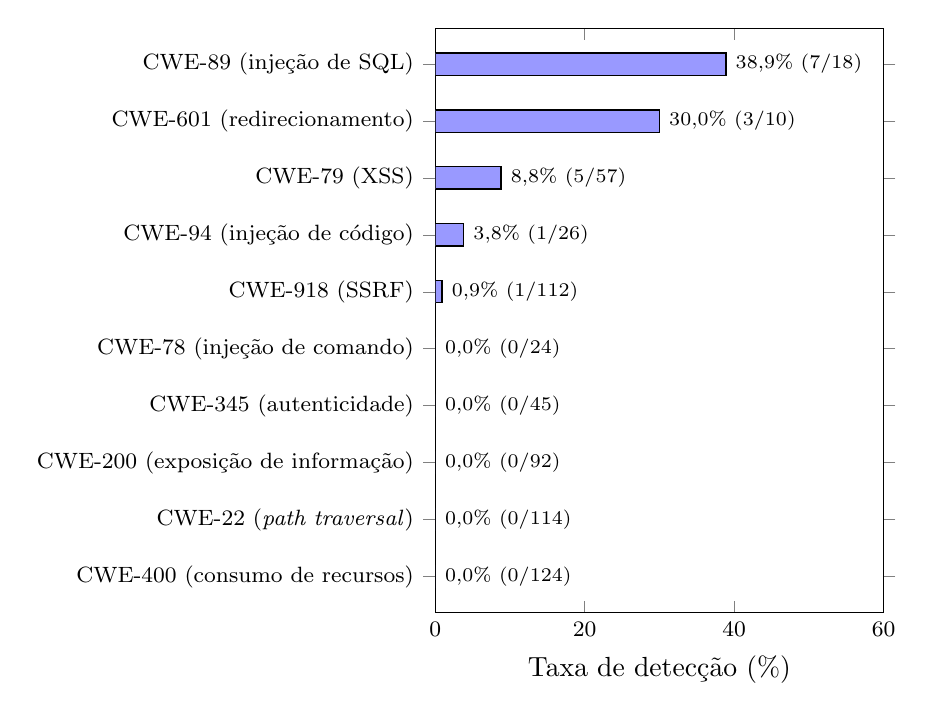
\begin{tikzpicture}
        \begin{axis}[
            xbar, xmin=0, xmax=60, width=0.6\textwidth, height=9cm,
            bar width=8pt, enlarge y limits=0.07,
            xlabel={Taxa de detecção (\%)},
            symbolic y coords={CWE-400,CWE-22,CWE-200,CWE-345,CWE-78,CWE-918,CWE-94,CWE-79,CWE-601,CWE-89},
            ytick=data,
            yticklabels={CWE-400 (consumo de recursos),CWE-22 (\textit{path traversal}),CWE-200 (exposição de informação),CWE-345 (autenticidade),CWE-78 (injeção de comando),CWE-918 (SSRF),CWE-94 (injeção de código),CWE-79 (XSS),CWE-601 (redirecionamento),CWE-89 (injeção de SQL)},
            tick label style={font=\footnotesize},
            nodes near coords,
            point meta=explicit symbolic,
            every node near coord/.append style={font=\scriptsize, anchor=west},
        ]
            \addplot[fill=blue!40] coordinates {
                (0.0,CWE-400) [0,0\% (0/124)]
                (0.0,CWE-22) [0,0\% (0/114)]
                (0.0,CWE-200) [0,0\% (0/92)]
                (0.0,CWE-345) [0,0\% (0/45)]
                (0.0,CWE-78) [0,0\% (0/24)]
                (0.9,CWE-918) [0,9\% (1/112)]
                (3.8,CWE-94) [3,8\% (1/26)]
                (8.8,CWE-79) [8,8\% (5/57)]
                (30.0,CWE-601) [30,0\% (3/10)]
                (38.9,CWE-89) [38,9\% (7/18)]
            };
        \end{axis}
    \end{tikzpicture}
    \fontepesquisa
\end{figure}

A figura mostra que o analisador funciona quando a fraqueza é visível no formato do código, numa única linha, e falha quando ela depende do caminho que um dado percorre pelo programa. A injeção de SQL em Go é o melhor exemplo do primeiro caso: a consulta montada com \texttt{fmt.Sprintf} e enviada ao banco tem um formato típico, o defeito cabe numa linha, e o código corrigido é visivelmente diferente. O redirecionamento aberto também se concentra num ponto único e reconhecível. O XSS é pouco detectado apesar de doze regras, porque elas cobrem só a forma mais típica do problema, enquanto o XSS real passa por \textit{frameworks} ou por APIs JSON. As duas maiores taxas, porém, vêm de amostras pequenas: 7 detecções em 18 pares e 3 em 10.

{\sloppy No extremo oposto estão as categorias mais numerosas, que são justamente as que o analisador não detecta: CWE-400, CWE-22, CWE-918 e CWE-200 somam 442 pares e uma única detecção. Na CWE-22 (\textit{path traversal}), as duas regras disponíveis cobrem apenas casos estreitos: o uso indevido de \texttt{filepath.Clean} e a extração de arquivo compactado. O caso geral, \texttt{os.Open(filepath.Join(base, entrada))}, tem a mesma forma na versão segura e na vulnerável. A diferença está em a entrada vir do usuário e não ter sido validada em outro ponto do programa, e isso o formato do código não mostra. Na CWE-918 (SSRF), a única regra acompanha o caminho do dado (análise de \textit{taint}), mas só dentro de um mesmo arquivo. A CWE-400 e a CWE-200 têm uma única regra cada.\par}

Dois fatos completam o quadro. Das 1.074 regras do \texttt{p/default}, apenas 84 se aplicam a Go. E nenhum dos alertas verificados trouxe o caminho do dado, mesmo quando se pediu à ferramenta que o registrasse, o que é coerente com a edição aberta do Semgrep, que só acompanha o dado dentro de um arquivo \cite{semgrepdocs}. A edição proprietária, que acompanha o dado entre arquivos, foi testada à parte e não detectou nenhum caso novo (Seção~\ref{subsec:h2}). Por que essas categorias não cedem é o assunto da Seção~\ref{sec:eliminacao}.

\subsection{Concorrência em Go: Ausência de Instrumento}
\label{subsec:q3concorrencia}

A Q3 previa atenção a fraquezas próprias de Go, entre elas as de concorrência. Verificou-se que as ferramentas usadas não conseguem medir essa classe, e isso é um resultado, e não uma lacuna da execução. A única categoria de concorrência presente no modo de filtro é a CWE-667 (bloqueio inadequado), com 14 alertas, todos de gabarito seguro. O especialista descartou os 14, e a acurácia de 100\% resultante não mede capacidade alguma.

A população tem, sim, casos vulneráveis de concorrência: 11 de CWE-362 (condição de corrida). Nenhum foi detectado pelo Semgrep, e por isso nenhum chegou ao modelo no modo de filtro. As fraquezas de concorrência em Go (condições de corrida, vazamento de \textit{goroutine}, canal não fechado) não são cobertas pelas regras sintáticas disponíveis, e as ferramentas efetivas para elas, como o detector de corrida da própria linguagem, operam por análise dinâmica \cite{tu2019understanding}. No modo de triagem, em que esses 11 casos chegam ao modelo, os modelos locais quase não os reconhecem: o especialista do \texttt{qwen2.5-coder:7b} reconheceu 2, e o do \texttt{gemma2:9b}, nenhum dos 8 que avaliou (os outros 3 ficaram sem veredito). O \texttt{gpt-6-luna} reconheceu 1 e 0 nas duas execuções sem raciocínio, e 6 e 8 com o raciocínio ligado, nos esforços baixo e alto. Esse último valor supera o \textit{recall} do mesmo modelo sobre o conjunto dos injetados (39\%), mas, com 11 casos e sem as versões seguras correspondentes entre os casos avaliados, não há como distinguir reconhecimento da fraqueza de tendência a responder ``vulnerável''. São números pequenos demais para uma leitura conclusiva.

Reunidas as três análises, a resposta à Q3 é parcial. O desempenho do modelo por categoria não pôde ser medido de forma confiável: a acurácia por CWE reflete mais quantos alertas seguros cada categoria tem do que a capacidade do modelo, e nenhuma categoria tem mais de sete casos vulneráveis. Quem decide o desempenho por categoria é o analisador, antes do modelo: ele detecta as fraquezas visíveis no formato do código, como a injeção de SQL, e quase nada nas que dependem do caminho do dado, que são justamente as mais numerosas. As fraquezas de concorrência, por fim, não puderam ser medidas. Os casos existem, mas o analisador não detecta nenhum, e por isso, no sistema implantado, nenhum chegaria ao modelo, por mais capaz que ele fosse. Responder a essa parte da pergunta exigiria um analisador com análise de concorrência, ou um componente dinâmico, e não apenas outro \textit{prompt} ou outro modelo.

% =============================================================================
\section{Q4: O Raciocínio do Modelo}
\label{sec:q4}

A Q4 pergunta de que forma a combinação de regras teóricas de segurança estruturadas em \textit{prompts} influencia a capacidade de raciocínio do modelo, e a metodologia associa a ela a auditoria qualitativa da justificativa que o modelo escreve antes do veredito: verificar se a decisão veio de uma fundamentação correta ou de alucinação. A auditoria não faz parte de nenhuma rodada de execução: foi conduzida depois, sobre os vereditos já gravados da Rodada 3, sem nova chamada ao modelo, porque o contexto entregue a ele em cada caso (o alerta do Semgrep, o trecho de código e o \textit{prompt}) pode ser remontado exatamente a partir dos resultados gravados da \textit{pipeline} (Seção~\ref{sec:arquitetura}).

\subsection{Protocolo}
\label{subsec:q4protocolo}

O critério de classificação foi escrito e registrado antes do sorteio da amostra e da leitura de qualquer caso. Cada justificativa é comparada com o código efetivamente entregue ao modelo e classificada em uma de três categorias:
\begin{itemize}
    \item \textbf{Fundada:} o argumento se apoia em elementos que existem no código, interpreta-os corretamente e, se for verdadeiro, sustenta o veredito.
    \item \textbf{Motivo errado:} nada é inventado, mas o argumento não sustenta o veredito, por ser genérico, circular, tratar de outra fraqueza, contradizer o próprio veredito ou interpretar mal um elemento que existe no código.
    \item \textbf{Alucinação:} o argumento afirma a existência de algo que não está no código, ou atribui a uma função da biblioteca padrão de Go um comportamento que ela não tem.
\end{itemize}

A categoria descreve a justificativa, e não o veredito: um veredito pode estar certo e ter sido justificado por motivo errado, e esse cruzamento é o que separa a última coluna da Tabela~\ref{tab:q4}. Para os alertas sobre código rotulado seguro que o modelo manteve, verificou-se ainda se o código, do jeito que foi entregue, era de fato seguro, vulnerável ou impossível de decidir só com aquele trecho. Esse resultado é apresentado na Seção~\ref{subsec:q4resultado}.

A amostra é de 25 casos, cada um lido nos dois \textit{prompts}, o que dá 50 vereditos. Os casos foram escolhidos a partir do resultado do especialista, de modo que os grupos pequenos, que são os mais informativos, não ficassem de fora: entram todos os 3 vulneráveis que ele reconheceu e todos os 12 alarmes falsos que ele manteve, e são sorteados, com semente fixa, 5 dos 16 vulneráveis que ele descartou e 5 dos 104 alertas que ele descartou e o \textit{baseline} manteve. Por isso, as proporções da amostra não devem ser lidas como estimativas para a população inteira.

Duas limitações acompanham o resultado e são declaradas aqui, e não apenas na Seção~\ref{sec:limitacoesresultados}. A classificação não é cega: quem classifica vê o veredito do modelo. E não há medida de concordância entre classificadores independentes: a classificação foi feita e revisada pelos próprios autores.

\subsection{Resultado}
\label{subsec:q4resultado}

A Tabela~\ref{tab:q4} resume a classificação. As três primeiras colunas dividem as 25 justificativas de cada \textit{prompt} pelas três categorias do protocolo. As duas últimas olham só para os vereditos certos: quantos foram no total e quantos deles vieram acompanhados de uma justificativa fundada.

\begin{table}[htpb]
    \centering
    \caption[Tipo de fundamento das justificativas auditadas]{Tipo de fundamento das justificativas na amostra auditada (25 casos por \textit{prompt}, Rodada 3)}
    \label{tab:q4}
    \renewcommand{\arraystretch}{1.4}
    \begin{tabular}{|l|c|c|c|c|c|}
        \hline
         & \multicolumn{3}{c|}{\textbf{Tipo de justificativa}} & \multicolumn{2}{c|}{\textbf{Vereditos certos}} \\
        \cline{2-6}
        \textbf{\textit{Prompt}} & \textbf{Fundada} & \textbf{Motivo errado} & \textbf{Alucinação} & \textbf{Total} & \textbf{Fundados} \\
        \hline
        \textit{Baseline} & 2 & 22 & 1 & 4 & 1 \\
        \hline
        Especialista & 4 & 18 & 3 & 8 & 4 \\
        \hline
    \end{tabular}
    \fontepesquisa
\end{table}

Dos 50 vereditos, 6 têm justificativa fundada, 40 têm motivo errado e 4 contêm alucinação. O especialista acerta mais vereditos que o \textit{baseline} na amostra (8 contra 4) e também justifica melhor os seus acertos: 4 dos seus 8 vereditos certos têm justificativa fundada, contra 1 dos 4 do \textit{baseline}. A outra justificativa fundada do \textit{baseline} acompanha um veredito contado como erro, num caso rotulado seguro de cópia sem limite de um arquivo compactado. O argumento descreve corretamente o código, e o erro é contra um gabarito que, nesse caso, não pode ser decidido a partir do trecho entregue (Seção~\ref{sec:limitacoesresultados}).

Três dos quatro acertos fundados do especialista estão no grupo de alertas que ele descartou e o \textit{baseline} manteve. Nesses casos, o argumento aponta que o MD5 ou o \texttt{math/rand} são usados para fins não criptográficos (chave de \textit{cache}, variação aleatória no tempo de expiração), que é exatamente o que a heurística da ficha da CWE manda verificar. É a forma positiva da influência perguntada pela Q4: quando a heurística se aplica ao caso, o raciocínio a segue e acerta pelo motivo certo. Ainda assim, a outra metade dos acertos do especialista na amostra vem com motivo errado ou com alucinação: o veredito está certo, mas a justificativa não o sustenta.

A leitura qualitativa revelou quatro padrões que as contagens sozinhas não mostram. O primeiro é a \textbf{repetição da mensagem do alerta}. Nos dez casos de CWE-614 da amostra (oito falsos e dois verdadeiros positivos do especialista), os dois \textit{prompts} afirmam que o \textit{cookie} é criado sem o atributo \texttt{Secure}, quando o código define \texttt{Secure} a partir de uma variável de configuração ou de uma função como \texttt{isTLS(r)}. A frase não é leitura do código, e sim a mensagem do Semgrep. O mesmo mecanismo produziu uma das alucinações: numa função que copia um arquivo compactado sem limite, o especialista afirma que o código usa \texttt{io.CopyN} para limitar a leitura. Essa função está na mensagem do alerta, e não no código. É a contraparte qualitativa do achado da Seção~\ref{subsec:q1controle}: a mensagem do Semgrep ocupa parte do lugar do código no raciocínio do modelo.

O segundo padrão é a \textbf{reprodução do exemplo da ficha}. Num caso de injeção de argumentos de processo, em que um valor vindo de fora chega aos argumentos de \texttt{exec.Command}, o especialista justifica o descarte com uma frase quase literal da justificativa do exemplo de falso positivo da ficha de CWE-94 (``a entrada externa é apenas dado interpolado, não código''), trocando ``\textit{template}'' por ``comando''. O enriquecimento semântico influencia o raciocínio também na forma negativa: o modelo reproduz o exemplo em vez de aplicá-lo.

O terceiro padrão é o \textbf{raciocínio certo com veredito oposto}: em dois casos de configuração de TLS, o especialista descreve corretamente o código como boa prática e, na mesma resposta, emite ``verdadeiro positivo''. A exigência de raciocínio antes do veredito, adotada na metodologia para estabilizar a resposta, não garante que o veredito decorra do raciocínio.

O quarto padrão diz respeito ao gabarito, e não ao modelo. Em dois pares de casos da amostra, o modelo recebeu \textbf{exatamente o mesmo recorte}, byte a byte, rotulado vulnerável na versão anterior à correção e seguro na versão corrigida: o \textit{commit} de correção alterou outra função do arquivo, e o alerta aponta para a mesma função nas duas versões. Com temperatura zero e semente fixa, o modelo necessariamente erra um dos dois. É a granularidade do rótulo, discutida na Seção~\ref{subsec:sobra}, vista do lado do componente neural.

Também sobre o gabarito, a auditoria verificou os 12 alertas sobre código rotulado seguro que o especialista manteve, para saber se o código, do jeito que foi entregue ao modelo, era de fato seguro. Seis eram de fato seguros, e nenhum era claramente vulnerável. Os outros seis não podiam ser decididos só com o trecho entregue. Em cinco deles, a segurança dependia de uma configuração definida fora da função. No sexto, havia dois padrões sem proteção, entre eles uma montagem de caminho de arquivo sem verificação, de outra CWE, cuja exploração depende da origem do arquivo. Entre os 5 alertas sorteados que só o \textit{baseline} manteve, os 5 eram seguros. Parte do gabarito negativo, portanto, não pode ser decidida olhando só uma função, o que delimita as métricas da Questão Geral (Seção~\ref{sec:limitacoesresultados}).

A resposta à Q4 é, portanto, que as regras de segurança colocadas no \textit{prompt} influenciam o raciocínio do modelo, mas nem sempre para melhor. Quando a heurística da ficha se aplica ao caso, o modelo a segue e acerta pelo motivo certo, como nos usos não criptográficos de MD5 e \texttt{math/rand}. Quando a ficha descreve uma situação diferente da do código, o modelo tende a copiar o exemplo dela em vez de analisar o caso: num alerta sobre os argumentos de \texttt{exec.Command}, o especialista justificou o descarte com a frase do exemplo da ficha de CWE-94, escrita para \textit{templates}. E, com os dois \textit{prompts}, o modelo muitas vezes repete a mensagem do alerta como se a tivesse lido no código. Na amostra, esses comportamentos predominam: apenas 6 das 50 justificativas são fundadas, e mesmo entre os acertos do especialista metade vem com justificativa errada. Isso reforça o que as métricas já indicavam: boa parte da redução de ruído vem de uma tendência geral a descartar alertas, e não de uma análise do código caso a caso.

% =============================================================================
\section{Por que o Teto de Detecção Não Cede}
\label{sec:eliminacao}

Esta seção investiga por que o Semgrep detecta tão poucos casos vulneráveis. Essa baixa detecção é o fator que mais limita os demais resultados, porque só os casos detectados chegam ao modelo no modo de filtro. Das 797 amostras de gabarito vulnerável, 19 receberam alerta na CWE do caso, ou 2,38\%. Esse número inclui, porém, fraquezas para as quais o \texttt{p/default} não tem nenhuma regra para Go, e que o Semgrep não poderia detectar de modo algum. Restrita às CWEs para as quais o \texttt{p/default} tem ao menos uma regra para Go, a taxa é de 18 em 690, ou 2,61\%, e é esse segundo número que interessa aqui.

Mesmo sobre esse denominador mais favorável, a taxa fica muito abaixo da reportada para analisadores estáticos sobre vulnerabilidades reais em Java, de 11,2\% a 26,5\% por ferramenta \cite{bennett2024semgrep}, comparação que a Figura~\ref{fig:recall-comparado} retoma na discussão. E ela não cede com mais coleta: uma coleta inicial de 257 pares rendeu 11 detecções (4,28\%), e triplicá-la, varrendo todas as 9.113 entradas de Go da base OSV, rendeu 18 (2,61\%). A taxa caiu, e não havia mais o que coletar.

A investigação dessa diferença ocupou quatro execuções sucessivas, cada uma dedicada a uma hipótese, e todas as hipóteses foram rejeitadas com medição própria. Esta seção as apresenta na ordem em que foram testadas, a mesma da Figura~\ref{fig:eliminacao}. As hipóteses H2 a H4 concentram-se nas duas maiores categorias cujo defeito depende do caminho do dado, CWE-22 e CWE-918, porque é nelas que a análise de fluxo e novas regras poderiam, em princípio, render detecções. A CWE-400 e a CWE-200, também numerosas, ficaram fora dessa investigação.

Rejeitadas as quatro, resta uma explicação que não depende do analisador, e sim da forma como o gabarito foi construído: a granularidade do rótulo e a abstração do código, apresentadas na Seção~\ref{subsec:sobra}. Uma hipótese sobre o componente neural, a de que as fichas do \textit{prompt} especialista, escritas por CWE e não por regra, limitassem o seu desempenho, foi testada depois e é discutida na Seção~\ref{subsec:q1fichas}.

\begin{figure}[htpb]
    \centering
    \caption[A cadeia de hipóteses testadas para o teto de detecção]{A cadeia de hipóteses testadas para a baixa detecção do Semgrep, na ordem em que foram testadas, e a explicação que restou}
    \label{fig:eliminacao}
    \begin{tikzpicture}[
        node distance=4mm,
        hip/.style={draw, rounded corners, align=left, font=\footnotesize, text width=100mm,
                    minimum height=12mm, inner sep=4pt, fill=black!4},
        sob/.style={hip, fill=green!12, very thick, draw=green!50!black},
        rej/.style={draw=red!70, text=red!70, font=\scriptsize\bfseries, rounded corners=1pt, inner sep=2pt},
        arr/.style={-{Latex[length=2mm]}, thick}
    ]
        \node[hip] (h1) {\textbf{H1: o conjunto de regras era o inadequado.}\\
            Medido: o \texttt{p/golang} tem 42 regras Go contra 84 do \texttt{p/default}, e deixava de produzir 97 alertas.};
        \node[hip, below=of h1] (h2) {\textbf{H2: faltava alcance ao motor de análise.}\\
            Medido: Semgrep Pro entre arquivos, 0 detecções novas em 5 casos; CodeQL, 3 de 47 arquivos.};
        \node[hip, below=of h2] (h3) {\textbf{H3: faltava regra pública.}\\
            Medido: 3 conjuntos públicos (\texttt{p/gosec}, \texttt{p/trailofbits}, \texttt{p/security-audit}): 0 regras Go novas para CWE-22 ou CWE-918.};
        \node[hip, below=of h3] (h4) {\textbf{H4: faltava regra própria.}\\
            Medido: 6,7\% (CWE-22) e 1,8\% (CWE-918) no grupo de avaliação.};
        \node[sob, below=6mm of h4] (s) {\textbf{O que sobra: granularidade do rótulo e abstração.}\\
            Medido: 25\% (CWE-22) e 48\% (CWE-918) dos arquivos rotulados não contêm a operação perigosa; 19\% e 30\% só a expõem atrás de abstração.};
        \foreach \h in {h1,h2,h3,h4}
            \node[rej, anchor=west] at ([xshift=2mm]\h.east) {REJEITADA};
        \draw[arr] (h1) -- (h2);
        \draw[arr] (h2) -- (h3);
        \draw[arr] (h3) -- (h4);
        \draw[arr] (h4) -- (s);
    \end{tikzpicture}
    \fonteautores
\end{figure}

\subsection{H1: o Conjunto de Regras Era o Inadequado}
\label{subsec:h1}

A primeira hipótese era que o conjunto de regras genérico \texttt{p/default} fosse a escolha errada, e que um conjunto específico para Go detectasse mais. O conjunto \texttt{p/golang} foi avaliado e recusado. Ele traz 42 regras, contra as 84 regras executáveis em Go dentro do \texttt{p/default}. Onze CWEs existem apenas no \texttt{p/default}, e as duas que existem apenas no \texttt{p/golang} não aparecem em nenhum caso da base de validação. Sobre a população, o \texttt{p/golang} deixava de produzir 97 alertas que o \texttt{p/default} produzia. Ser específico para Go, portanto, não significa cobrir mais, e a hipótese foi rejeitada.

\subsection{H2: Faltava Alcance ao Motor de Análise}
\label{subsec:h2}

A segunda hipótese atribuía a não-detecção à ausência de análise de fluxo entre arquivos. Ela foi testada por dois caminhos. No primeiro, executou-se a edição proprietária do Semgrep, que analisa o fluxo entre arquivos e estava disponível em plano gratuito, com o repositório inteiro em análise e o mesmo critério de detecção da execução normal (alerta na CWE do caso), sobre casos das duas categorias mais numerosas sem detecção, CWE-22 e CWE-918.

Em nenhum dos 5 casos com resultado (3 de CWE-22 e 2 de CWE-918) houve detecção nova, e um sexto caso excedeu o tempo limite de 900 segundos. O tempo de execução foi de 2 a 5 vezes maior que o da edição aberta: no repositório \texttt{1panel}, por exemplo, a edição aberta emitiu 60 alertas no repositório inteiro, em 55,9 segundos, e a proprietária, 63 alertas, em 123,7 segundos, mas nenhuma das duas alertou o arquivo do caso, que continuou não detectado. Nos cinco casos, nem a edição aberta nem a proprietária emitiram qualquer alerta sobre o arquivo do gabarito: o que falta ali é uma regra que examine esse arquivo, e alcance entre arquivos não conserta arquivo que regra nenhuma examina.

No segundo caminho, o CodeQL, que analisa o fluxo de dados entre funções e entre arquivos, foi executado sobre 81 casos vulneráveis não detectados pelo Semgrep, restritos às categorias que dependem do caminho do dado e deliberadamente escolhidos no cenário mais favorável ao CodeQL. Como vários casos caem no mesmo arquivo, o resultado é contado por arquivo: são 47 arquivos de 14 repositórios, dos quais o CodeQL recuperou 3 (6,4\%). O resultado separa as duas categorias. Na CWE-22, recuperou 2 de 8 arquivos, o que confirma que a análise de fluxo tira essa categoria do zero. Na CWE-918, recuperou 1 de 29, o que refuta a hipótese para ela. Como verificação adicional, o SonarQube, em edição comunitária, não recuperou nenhum caso, por não possuir regra de segurança para Go.

Duas ressalvas limitam o alcance dessa conclusão. O teste do Semgrep Pro cobriu 5 casos, escolhidos em intervalos regulares da lista de casos, e não por sorteio, e o tempo limite mostra que repositórios grandes ficam sub-representados. O do CodeQL cobriu 81 casos, numa amostra escolhida por conveniência. A diferença de tamanho entre as duas amostras vem do custo de cada ferramenta: o CodeQL constrói uma base por repositório e avalia de uma vez todos os casos dele, e a amostra foi concentrada em 14 repositórios pequenos, enquanto o teste do Semgrep Pro analisava o repositório inteiro a cada caso, sob o limite de 900 segundos. Os dois testes bastam para descartar a reexecução da população inteira com outra ferramenta, mas não para afirmar que a análise entre arquivos não ajudaria em geral.

A falta de análise entre arquivos explica, portanto, uma parte pequena da não-detecção, e não a maior parte dela: o CodeQL recuperou alguns casos, sobretudo de CWE-22, mas, dos 47 arquivos testados, 44 continuaram sem detecção nas três ferramentas (Semgrep, CodeQL e SonarQube). Por isso, a hipótese foi rejeitada como explicação principal.

\subsection{H3: Faltava Regra em Outro Conjunto Público}
\label{subsec:h3}

A terceira hipótese era que regras sintáticas para as duas categorias, CWE-22 e CWE-918, existissem em outro conjunto público do repositório de regras do Semgrep, em particular as do \textit{gosec}, um analisador de segurança próprio para Go, cujas regras foram reescritas no formato do Semgrep e não dependeriam de fluxo. Três conjuntos foram inspecionados regra por regra: \texttt{p/gosec} (23 regras, todas para Go), \texttt{p/trailofbits} (120 regras, 18 para Go) e \texttt{p/security-audit} (225 regras, 28 para Go). Nenhum acrescenta regra Go para CWE-22 ou CWE-918 além das já presentes no \texttt{p/default}. Estendida a todas as CWEs dos casos vulneráveis da população, a inspeção encontrou uma única regra nova, do \texttt{p/trailofbits}, para a CWE-1284, específica de nós da rede Ethereum, numa categoria com apenas 2 casos vulneráveis.

Apesar do nome, o conjunto \texttt{p/gosec} disponível no repositório do Semgrep não traz as regras do \textit{gosec} reescritas: é uma seleção de regras do próprio Semgrep, das quais 22 de 23 já constam do \texttt{p/default}. As regras do \textit{gosec} para as duas fraquezas, G304 (caminho de arquivo) e G107 (URL de requisição), não estão nele, e a única regra exclusiva trata de uma fraqueza ausente da população. A hipótese foi rejeitada. O que ela mede é a oferta de regras públicas, e não a ferramenta: o que se afirma é que os conjuntos públicos disponíveis não trazem regra nova, e não que o Semgrep seja incapaz de detectar essas fraquezas.

Fica de fora desta verificação o \textit{gosec} autônomo, que tem regras sintáticas para os dois casos (G304, para caminho de arquivo, e G107, para URL de requisição) e não foi executado. Como essas regras alertam qualquer abertura de arquivo ou requisição com destino variável, e a versão corrigida dos casos de CWE-22 costuma ter a mesma forma da vulnerável (Seção~\ref{subsec:q3secas}), é provável que alertassem também as versões corrigidas, sem distinguir uma da outra. A verificação fica como trabalho futuro.

\subsection{H4: Faltava Regra Própria}
\label{subsec:h4}

Restava escrever regras próprias. O risco era evidente: uma regra escrita olhando para os casos em que será medida descreve esses casos, e não a fraqueza, e tende a acertar só eles. Por isso, o procedimento foi fixado antes de qualquer medição. Os casos das duas categorias foram divididos em dois grupos fixos: um de \textbf{desenvolvimento}, que podia ser consultado ao escrever as regras, e um de \textbf{avaliação}, reservado para medi-las. A divisão foi registrada no histórico do repositório do projeto (Apêndice~\ref{ap:repositorio}), num \textit{commit} anterior ao da primeira regra, de modo que a ordem pode ser verificada, e não apenas afirmada.

Foram escritos dois tipos de regra. As \textbf{derivadas da definição} usam apenas a definição da CWE e a documentação de Go, sem olhar caso algum, e por isso podem ser medidas sobre a população inteira. As \textbf{informadas pelos casos} foram escritas consultando o grupo de desenvolvimento, e por isso só podem ser medidas no grupo de avaliação.

As regras derivadas da definição detectaram 2 de 114 casos de CWE-22 (1,8\%) e 1 de 112 de CWE-918 (0,9\%). Com todas as regras, no grupo de avaliação, a detecção foi de 4 em 60 (6,7\%) em CWE-22 e de 1 em 57 (1,8\%) em CWE-918. No grupo de desenvolvimento, que serve apenas para diagnóstico, já que as regras foram escritas olhando para ele, os valores foram de 7,4\% e 5,5\%. Em CWE-22, os dois grupos quase coincidem, porque a regra de extração de arquivo compactado descreve um padrão de código comum e, por isso, vale também para casos não vistos. Em CWE-918, o desenvolvimento é três vezes a avaliação, porque ali a regra descreve mais os casos vistos do que a fraqueza.

A base estatística é frágil: no grupo de avaliação há 60 casos de CWE-22 e 57 de CWE-918, dos quais as regras detectaram apenas 4 e 1, respectivamente. Com contagens tão pequenas, um único caso a mais ou a menos muda bastante a taxa (em CWE-918, uma detecção a mais a dobraria, de 1,8\% para 3,5\%), e por isso os números servem para descrever ordem de grandeza, e não para afirmar a superioridade de uma configuração. Resta ainda uma ameaça: a divisão garante que os números não foram inflados pelas regras, mas não que a escolha das categorias seja neutra, porque CWE-22 e CWE-918 foram escolhidas justamente depois de se ver que eram as que menos detectavam. Como em \citeonline{bennett2024semgrep}, a contribuição está na análise das lacunas das regras, e não no conjunto de regras resultante. A hipótese foi rejeitada: regra própria melhora pouco a detecção, e o motivo é o assunto da próxima subseção.

\subsection{O que Sobra: Granularidade do Rótulo e Abstração}
\label{subsec:sobra}

As quatro hipóteses anteriores foram rejeitadas, e a explicação que restou está na forma como o gabarito foi construído. O rótulo é dado por arquivo (Seção~\ref{subsec:base}). A \textbf{granularidade} do rótulo é o tamanho da porção de código a que ele se aplica: neste trabalho, o arquivo inteiro, e não uma função ou uma linha. O \textbf{arquivo rotulado} como vulnerável é o arquivo que o \textit{commit} de correção alterou. Esse arquivo, porém, é com frequência aquele em que a verificação foi \textbf{acrescentada}, e não aquele em que a operação perigosa se encontra. A Figura~\ref{fig:rotulo} ilustra o mecanismo de forma esquemática.

\begin{figure}[htpb]
    \centering
    \caption[Granularidade do rótulo: o arquivo rotulado e a operação perigosa]{Por que o arquivo rotulado pode não conter a operação perigosa: o \textit{commit} de correção acrescenta a verificação em um arquivo, e a operação está em outro (exemplo esquemático)}
    \label{fig:rotulo}
    \resizebox{\textwidth}{!}{
    \begin{tikzpicture}[
        cod/.style={draw, rounded corners, align=left, font=\scriptsize\ttfamily, inner sep=4pt, text width=74mm},
        tit/.style={font=\footnotesize\bfseries, align=center},
        arr/.style={-{Latex[length=2mm]}, thick}
    ]
        \node[cod, fill=red!6, anchor=north] (a) at (0,0) {%
func Baixar(w http.ResponseWriter, r *http.Request) \{\\
\ \ nome := r.URL.Query().Get("arquivo")\\
\textcolor{green!45!black}{+ if strings.Contains(nome, "..") \{}\\
\textcolor{green!45!black}{+ \ \ http.Error(w, "inválido", 400)}\\
\textcolor{green!45!black}{+ \ \ return}\\
\textcolor{green!45!black}{+ \}}\\
\ \ s.armazenamento.Ler(nome)\\
\}};
        \node[cod, fill=black!3, anchor=north] (b) at (9.0,0) {%
func (s *Armazenamento) Ler(nome string) \{\\
\ \ caminho := filepath.Join(s.base, nome)\\
\ \ f, err := \textbf{os.Open(caminho)}\\
\ \ ...\\
\}};
        \node[tit, anchor=south west] at ([yshift=1mm]a.north west) {handler.go};
        \node[draw=red!70, text=red!70, font=\scriptsize\bfseries, anchor=south east] at ([yshift=1mm]a.north east) {GABARITO: VULNERÁVEL};
        \node[tit, anchor=south west] at ([yshift=1mm]b.north west) {storage.go};
        \node[font=\scriptsize, text=black!60, anchor=south east] at ([yshift=1mm]b.north east) {não tocado pelo \textit{commit}};

        \node[draw, rounded corners, fill=blue!10, font=\scriptsize, align=center] (regra) at ([shift={(4.5,-2.2)}]a.south) {regra: procura \texttt{os.Open(...)} \\ com caminho montado da entrada};
        \draw[arr, red!70, dashed] (regra.north west) -- node[left=2mm, font=\scriptsize, align=right] {nada a casar\\no arquivo rotulado} (a.south);
        \draw[arr, green!45!black] (regra.north east) -- node[right=2mm, font=\scriptsize, align=left] {casaria aqui,\\fora do rótulo} (b.south);
        \node[font=\scriptsize, text=green!45!black, align=left, anchor=north west] at ([yshift=-2mm]a.west |- regra.south) {+ linhas acrescentadas pelo \textit{commit} de correção};
    \end{tikzpicture}
    }
    \fonteautores
\end{figure}

Para medir com que frequência isso acontece, os arquivos rotulados foram lidos um a um. Em todos os 226 casos vulneráveis das duas categorias (114 de CWE-22 e 112 de CWE-918), foi verificado se o arquivo rotulado contém a operação perigosa e de que forma. Nos 109 casos do grupo de desenvolvimento (Seção~\ref{subsec:h4}), foi verificado também de onde vem o dado que chega a ela. A Tabela~\ref{tab:lacuna} mostra o primeiro ponto: classifica cada caso pela forma como a operação perigosa aparece no arquivo rotulado, e cada caso cai em exatamente uma das três linhas. Cada valor é a porcentagem dos casos daquela CWE: na primeira linha, por exemplo, 55,3\% em CWE-22 são 63 dos 114 casos dessa categoria. O segundo ponto, a origem do dado, é tratado mais adiante, na Tabela~\ref{tab:origem}.

\begin{table}[htpb]
    \centering
    \caption[Forma da operação perigosa no arquivo rotulado]{Forma em que a operação perigosa aparece no arquivo rotulado, em todos os casos vulneráveis das duas categorias, em porcentagem dos casos de cada CWE (entre parênteses, o número de casos)}
    \label{tab:lacuna}
    \renewcommand{\arraystretch}{1.4}
    \setlength{\tabcolsep}{4pt}
    \small
    \begin{tabular}{|l|c|c|}
        \hline
        \textbf{Observação} & \textbf{CWE-22 (114)} & \textbf{CWE-918 (112)} \\
        \hline
        Operação chamada diretamente (\texttt{os.Open}, \texttt{http.Get}) & 55,3\% & 21,4\% \\
        \hline
        Operação só atrás de abstração & 19,3\% & 30,4\% \\
        \hline
        Sem operação perigosa no arquivo rotulado & 25,4\% & 48,2\% \\
        \hline
    \end{tabular}
    \fontepesquisa
\end{table}

Para 25,4\% dos casos de CWE-22 e 48,2\% dos de CWE-918, portanto, nenhuma regra sintática, pública ou própria, poderia detectar no arquivo rotulado uma operação que não está nele. A não detecção desses casos não diz nada sobre o analisador: diz sobre onde o rótulo foi colocado. Quando a operação existe, ela aparece com frequência atrás de uma abstração: em vez de chamar diretamente a biblioteca padrão de Go, o código usa uma biblioteca de terceiros que oferece a mesma operação (como \texttt{afero} e \texttt{billy}, que imitam o sistema de arquivos), a interface genérica de arquivos da própria linguagem (\texttt{fs.FS}) ou um método do próprio projeto que embrulha o cliente HTTP. Isso ocorre em 19,3\% dos casos de CWE-22 e em 30,4\% dos de CWE-918, e uma regra que procura a chamada à biblioteca padrão não casa com esses casos, como mostra a Figura~\ref{fig:abstracao}.

\begin{figure}[htpb]
    \centering
    \caption[A operação perigosa atrás de abstração]{A mesma operação, direta e atrás de abstração: a regra que nomeia a biblioteca padrão casa com a primeira e não com a segunda}
    \label{fig:abstracao}
    \resizebox{0.9\textwidth}{!}{
    \begin{tikzpicture}[
        cod/.style={draw, rounded corners, align=left, font=\scriptsize\ttfamily, inner sep=4pt, text width=60mm, minimum height=14mm},
        arr/.style={-{Latex[length=2mm]}, thick}
    ]
        \node[draw, rounded corners, fill=blue!10, font=\scriptsize, align=center] (regra) at (4,2.2) {padrão da regra: \texttt{os.Open(\$CAMINHO)}};
        \node[cod, fill=black!3] (a) at (0,0) {%
caminho := filepath.Join(base, nome)\\
f, err := os.Open(caminho)};
        \node[cod, fill=black!3] (b) at (8,0) {%
var fs afero.Fs = afero.NewOsFs()\\
caminho := filepath.Join(base, nome)\\
f, err := fs.Open(caminho)};
        \draw[arr, green!45!black] (regra) -- node[above left=1pt, font=\scriptsize] {casa} (a.north);
        \draw[arr, red!70, dashed] (regra) -- node[above right=1pt, font=\scriptsize] {não casa} (b.north);
        \node[font=\scriptsize, below=1mm of a] {chamada direta à biblioteca padrão};
        \node[font=\scriptsize, below=1mm of b] {mesma operação, por interface de terceiros};
    \end{tikzpicture}
    }
    \fonteautores
\end{figure}

\begin{table}[htpb]
    \centering
    \caption[Origem do dado que chega à operação perigosa]{Origem do dado que chega à operação perigosa, nos casos vulneráveis do grupo de desenvolvimento, em porcentagem dos casos de cada CWE (um mesmo caso pode aparecer em mais de uma linha)}
    \label{tab:origem}
    \renewcommand{\arraystretch}{1.4}
    \small
    \begin{tabular}{|l|c|c|}
        \hline
        \textbf{Observação} & \textbf{CWE-22 (54)} & \textbf{CWE-918 (55)} \\
        \hline
        Arquivo lê parâmetro de requisição HTTP & 11,1\% & 23,6\% \\
        \hline
        Parâmetro HTTP e operação no mesmo arquivo & 5,6\% & 14,5\% \\
        \hline
        Dado vem de campo de \textit{struct} & 42,6\% & 67,3\% \\
        \hline
    \end{tabular}
    \fontepesquisa
\end{table}

Por fim, a origem do dado raramente é a que a definição da CWE sugere. A definição descreve um dado vindo do usuário, o que, num serviço web, costuma significar um parâmetro lido da requisição HTTP (por exemplo, \texttt{r.URL.Query().Get("arquivo")}), e as regras derivadas da definição exigem essa origem. Mas, como mostra a Tabela~\ref{tab:origem}, no grupo de desenvolvimento só 11,1\% dos casos de CWE-22 e 23,6\% dos de CWE-918 leem algum parâmetro de requisição no arquivo rotulado, e só 5,6\% e 14,5\% têm, no mesmo arquivo, a leitura do parâmetro e a operação perigosa, que é o que uma regra de arquivo único precisa ver.

Na maioria dos casos, o dado chega por um campo de \textit{struct}, isto é, um atributo de um objeto preenchido em outro ponto do programa, por exemplo a partir de um JSON recebido (42,6\% e 67,3\%). Em CWE-22, boa parte dos casos é de extração de arquivo compactado (20,4\% dos casos trazem código desse tipo): o dado externo é o nome de um arquivo dentro do pacote, e não um parâmetro de requisição. Saber se um campo de \textit{struct} carrega dado do usuário exige acompanhar o programa até o ponto em que o campo foi preenchido, e as ferramentas de análise de fluxo só começam esse acompanhamento a partir de origens que reconhecem como entrada do usuário, como os parâmetros de uma requisição. Um campo preenchido por um \textit{framework}, por uma mensagem decodificada ou pelo estado de uma tarefa não é reconhecido como origem, a menos que alguém o declare à ferramenta. Isso ajuda a entender por que nem o CodeQL, que acompanha o dado entre arquivos, recuperou a CWE-918 (1 de 29 arquivos, Seção~\ref{subsec:h2}).

{\sloppy Isso não é um defeito específico da forma como a base deste trabalho foi montada, e sim uma propriedade conhecida das bases de vulnerabilidades derivadas de \textit{commits} de correção: o \textit{commit} indica apenas aproximadamente onde está a falha, e quanto dessa imprecisão passa para o gabarito depende da granularidade escolhida para o rótulo, aqui o arquivo \cite{croft2023dataquality, bhandari2021cvefixes}. A contribuição deste trabalho é medir essa imprecisão para Go, nas duas categorias que concentram a perda (Tabela~\ref{tab:lacuna}). A medida cobre todos os casos vulneráveis dessas duas categorias, mas não as demais, e a origem do dado (Tabela~\ref{tab:origem}) foi verificada apenas no grupo de desenvolvimento.\par}

Reunidas as análises, a resposta à pergunta desta seção é que o teto de detecção não decorre principalmente da ferramenta escolhida nem da falta de regras. Trocar o conjunto de regras, ampliar o alcance da análise ou escrever regras próprias rendeu pouco ou nada (H1 a H4). O que mais limita a detecção é a forma como o gabarito foi construído: em 25,4\% dos casos de CWE-22 e 48,2\% dos de CWE-918, o arquivo rotulado nem contém a operação perigosa, e, quando a contém, ela aparece com frequência atrás de abstração ou depende de um dado vindo de outro ponto do programa. A baixa detecção do Semgrep não deve, por isso, ser lida apenas como fraqueza do analisador: parte dela é um limite da própria medição.

% =============================================================================
\section{Análise Comparativa dos Modelos}
\label{sec:modelos}

Esta seção compara os três modelos avaliados: os dois locais, \texttt{qwen2.5-coder:7b} e \texttt{gemma2:9b}, e o comercial, \texttt{gpt-6-luna}, com e sem raciocínio. A pergunta é se as conclusões das seções anteriores, obtidas sobretudo com o \texttt{qwen2.5-coder:7b}, dependem do modelo: um modelo maior ou mais capaz filtraria melhor os alertas, ou recuperaria mais casos que o analisador perde? A seção compara primeiro os dois modelos locais, depois o modelo comercial e, por fim, o mesmo modelo comercial com o raciocínio ligado.

\subsection{Os Dois Modelos Locais}
\label{subsec:modeloslocais}

{\sloppy A Rodada 6 trocou o modelo e manteve todo o resto: a pergunta direta, a população, a semente e a temperatura. O \texttt{gemma2:9b} tem mais parâmetros que o \texttt{qwen2.5-coder:7b}, e a pergunta era se um modelo maior recuperaria mais dos casos que o analisador perde (Seção~\ref{subsec:q2triagem}). A rodada comercial repetiu o mesmo modo e a mesma pergunta com o \texttt{gpt-6-luna}. A Tabela~\ref{tab:modelos} reúne os três modelos no modo de triagem.\par}

\begin{table}[htpb]
    \centering
    \caption[Comparação entre modelos, por origem]{Comparação entre modelos no modo de triagem, com a pergunta direta, separada pela origem dos casos. Todas as linhas avaliam os mesmos casos: os modelos locais na segunda execução das Rodadas 5 e 6, e o comercial em duas execuções (quando as duas diferem, os dois valores são dados). A pilha tem 22 vulneráveis nas linhas do \textit{baseline} e 21 nas do especialista}
    \label{tab:modelos}
    \renewcommand{\arraystretch}{1.4}
    \setlength{\tabcolsep}{3pt}
    \footnotesize
    \begin{tabular}{|l|c|c|c|c|}
        \hline
         & \multicolumn{3}{c|}{\textbf{Pilha de alertas}} & \textbf{Injetados} \\
        \cline{2-5}
        \textbf{Configuração} & \textbf{\textit{Recall}} & \textbf{Precisão} & \textbf{MCC} & \textbf{\textit{Recall}} \\
        \hline
        \texttt{qwen2.5-coder:7b}, especialista direto & 14,29\% & 7,14\% & $+0{,}068$ & 4,08\% \\
        \hline
        \texttt{gemma2:9b}, especialista direto & 38,10\% & 7,08\% & $+0{,}115$ & 6,52\% \\
        \hline
        \texttt{qwen2.5-coder:7b}, \textit{baseline} direto & 9,09\% & 6,25\% & $+0{,}045$ & 1,19\% \\
        \hline
        \texttt{gemma2:9b}, \textit{baseline} direto & 40,91\% & 2,60\% & $-0{,}002$ & 23,65\% \\
        \hline
        \texttt{gpt-6-luna}, especialista direto & 71,43\% & 15,00--15,46\% & $+0{,}294$ / $+0{,}299$ & 17,12--17,26\% \\
        \hline
        \texttt{gpt-6-luna}, \textit{baseline} direto & 59,09--63,64\% & 7,26--7,87\% & $+0{,}151$ / $+0{,}170$ & 17,57--17,97\% \\
        \hline
    \end{tabular}
    \fontepesquisa
\end{table}

A tabela separa os casos pela origem, porque cada origem mede uma tarefa diferente. Na pilha de alertas, quase toda de código seguro, o modelo precisa separar os poucos vulneráveis do ruído. Por isso a tabela traz o \textit{recall} (a fração dos vulneráveis reconhecidos), a precisão (a fração dos vereditos ``vulnerável'' que estavam certos) e o MCC. Nos injetados, todos vulneráveis, só o \textit{recall} faz sentido (Seção~\ref{subsec:q2triagem}). Juntar as duas origens produziria uma população com cerca de 50\% de vulneráveis, que não corresponde a nenhum uso real, e por isso as métricas do modo de triagem como um todo não são usadas aqui.

Todos os valores da tabela vêm da mesma base de casos. Para os modelos locais, são os da segunda execução das Rodadas 5 e 6, feita justamente para permitir a comparação caso a caso com as rodadas posteriores, e por isso diferem um pouco dos das Tabelas~\ref{tab:filtro} e~\ref{tab:triagem}. Nessa base, a pilha tem 22 casos vulneráveis, e não os 19 da Rodada 3, porque três pares de casos de CWE-22 de um mesmo repositório passaram a receber alerta nas duas versões, a vulnerável e a corrigida. Nas linhas do especialista, são 21, porque um caso ficou sem veredito válido em um dos modelos.

{\sloppy Trocar o modelo local por um maior não aumentou muito a recuperação desses casos. Com o especialista, o \texttt{gemma2:9b} recupera 6,52\% dos injetados, contra 4,08\% do \texttt{qwen2.5-coder:7b}, uma diferença pequena. Com o \textit{baseline}, o \texttt{gemma2:9b} reconhece mais injetados que o \texttt{qwen2.5-coder:7b} (23,65\% contra 1,19\%), mas pelo motivo já apontado na Seção~\ref{subsec:q2triagem}: viés de resposta. Ele responde ``vulnerável'' com muito mais frequência, seja o código vulnerável ou seguro. Na pilha, o seu \textit{baseline} marca como vulneráveis 337 alertas seguros, contra 30 do \texttt{qwen2.5-coder:7b}, e a sua precisão, de 2,6\%, é a mesma proporção de vulneráveis que há na pilha: é o que se obteria respondendo ao acaso. Esse comportamento se repete nas duas execuções.\par}

Já a comparação dos dois modelos pelo MCC na pilha não se sustenta. Na tabela, o \texttt{gemma2:9b} tem MCC maior com o especialista ($+0{,}115$ contra $+0{,}068$) e menor com o \textit{baseline} ($-0{,}002$ contra $+0{,}045$). Na primeira execução das mesmas rodadas, contados só os 18 vulneráveis em que os dois modelos deram veredito válido, ele tinha MCC menor com os dois \textit{prompts}: no especialista, por exemplo, $+0{,}108$ contra $+0{,}159$. Na Tabela~\ref{tab:filtro}, o \texttt{qwen2.5-coder:7b} aparece com $+0{,}188$ porque ali conta os 19 vulneráveis. Com cerca de 20 vulneráveis na pilha, a variação entre duas execuções da mesma configuração basta para inverter a ordem dos modelos. Por isso, essas diferenças não permitem dizer qual deles discrimina melhor.

No modo de filtro, a comparação é mais clara e desfavorável ao modelo maior. Ali, os dois modelos foram executados nas mesmas condições, sobre os mesmos 822 casos (Tabela~\ref{tab:filtro}). As linhas do \texttt{gemma2:9b} vêm da sétima rodada, na execução com o catálogo de fichas por CWE, o mesmo das demais rodadas. Com o especialista, o \texttt{qwen2.5-coder:7b} acerta mais: em 176 casos só ele acerta, contra 16 em que só o \texttt{gemma2:9b} acerta ($p < 0{,}0001$). Com o \textit{baseline}, os dois não se distinguem (97 contra 82, $p = 0{,}30$). É também no \texttt{gemma2:9b} que o enriquecimento semântico deixa de ajudar no filtro (Seção~\ref{subsec:q1pareado}).

{\sloppy A ressalva é obrigatória: o \texttt{gemma2:9b} não é uma versão maior do \texttt{qwen2.5-coder:7b}. Entre os dois mudam, ao mesmo tempo, a família do modelo, a especialização (o \texttt{gemma2:9b} é generalista, e o \texttt{qwen2.5-coder:7b}, especializado em código) e a quantização (Seção~\ref{sec:limitacoes}). O resultado mostra que \textit{este} modelo maior não superou um modelo menor especializado em código. Não mostra que um modelo maior não ajude.\par}

\subsection{O Modelo Comercial}
\label{subsec:modelocomercial}

A rodada comercial verificou até onde as conclusões obtidas com os modelos locais se estendem a um modelo comercial. O \texttt{gpt-6-luna} foi executado sem raciocínio e com temperatura zero, nos dois modos, sobre a mesma população e com os mesmos \textit{templates} e catálogo de fichas. Como o modelo não oferece semente fixa, cada modo foi executado duas vezes. As duas execuções deram o mesmo veredito em 97,4\% a 99,1\% dos casos, conforme o modo, com $\kappa$ de Cohen entre 0,935 e 0,969 (Seção~\ref{sec:plano}), perto do máximo de 1. Repetir a execução muda poucos vereditos, mas, quando a diferença entre duas configurações depende de poucos casos, isso basta para alterar a conclusão, como se vê adiante no modo de filtro. As chamadas foram feitas pela interface de lote do fornecedor, que processa os pedidos de forma assíncrona e a preço menor, e o custo total foi de US\$~1,15.

O resultado não é o mesmo nos dois modos. Em parte, isso se explica de novo pelo viés de resposta: o modelo comercial responde ``vulnerável'' com muito mais frequência que os locais.

No modo de triagem, isso o torna o melhor dos três modelos. Com o especialista direto, ele reconhece 15 dos 21 vulneráveis da pilha de alertas, com precisão de cerca de 15\% e MCC de $+0{,}29$ a $+0{,}30$, contra $+0{,}068$ e $+0{,}115$ dos modelos locais (Tabela~\ref{tab:modelos}). Entre os injetados, recupera de 17,12\% a 17,26\%, contra 4,08\% e 6,52\%. O teste de McNemar favorece o modelo comercial contra cada modelo local, nas duas execuções ($p < 0{,}0001$).

Diferentemente do que ocorre com o \textit{baseline} do \texttt{gemma2:9b}, esse ganho não vem apenas de responder ``vulnerável'' com mais frequência. O \textit{baseline} direto do modelo comercial tem cerca de metade dos alarmes falsos do \textit{baseline} do \texttt{gemma2:9b} (164 a 166, contra 337) e, ainda assim, MCC de $+0{,}15$ a $+0{,}17$ na pilha, contra $-0{,}002$. A vantagem do especialista sobre o \textit{baseline} também se repete nas duas execuções: em 189 casos só o especialista acerta, contra 110 em que só o \textit{baseline} acerta, na primeira, e 187 contra 105 na segunda ($p < 0{,}0001$ nas duas).

No modo de filtro, o mesmo viés o torna um filtro pior. Sobre os mesmos 820 a 822 casos, ele descarta de 66\% a 70\% dos alertas, contra 85\% e 98\% do \texttt{qwen2.5-coder:7b} com o \textit{baseline} e com o especialista, e mantém de 240 a 269 alarmes falsos, contra 115 e 12. Ele reconhece mais vulneráveis (9 dos 19 com o \textit{baseline}, 10 e 12 com o especialista, nas duas execuções), mas, numa pilha quase toda segura, isso não compensa os alarmes a mais. O MCC fica entre $+0{,}056$ e $+0{,}097$, abaixo do $+0{,}116$ e do $+0{,}161$ do \texttt{qwen2.5-coder:7b}, próximo do $+0{,}043$ e acima do $-0{,}002$ do \texttt{gemma2:9b}.

Como no \texttt{gemma2:9b}, o especialista não ajuda o modelo comercial no filtro. A diferença para o \textit{baseline} é significativa em uma execução ($p = 0{,}032$) e não na outra ($p = 0{,}227$). Os alarmes falsos que o especialista acrescenta se concentram na CWE-327 (57 e 54 nas duas execuções, contra 19 e 20 do \textit{baseline}), a mesma categoria em que a ficha por CWE descreve uma fraqueza diferente da apontada pelo alerta (Seção~\ref{subsec:q1pareado}).

A comparação mede um único modelo comercial, de faixa econômica, escolhido por ser o que uma equipe empregaria para triar alertas em volume. Um relato ainda não revisado por pares sugere que modelos dessa faixa alcançam, na triagem de alertas, acurácia comparável à de modelos de topo de linha \cite{alatasi2026aisast}, mas modelos de topo de linha não foram medidos aqui. O mesmo modelo com o raciocínio ligado foi medido, e é o assunto da próxima subseção.

\subsection{O Modelo Comercial com Raciocínio}
\label{subsec:raciocinio}

O \texttt{gpt-6-luna} foi executado novamente com o raciocínio ligado, isto é, com permissão para gerar uma etapa de raciocínio interna antes da resposta, em dois níveis de esforço, baixo e alto, nos dois modos e com os dois \textit{prompts}. Com o raciocínio ligado, a interface do fornecedor não aceita temperatura zero, e as chamadas saíram na temperatura padrão. Mudam, assim, duas coisas ao mesmo tempo: o raciocínio e a temperatura. Por restrição de orçamento, cada configuração foi executada uma única vez. Ainda assim, as diferenças medidas não se confundem com a variação entre execuções: entre o modelo sem e com raciocínio, mudam de sete a dezesseis vezes mais vereditos do que entre as duas execuções sem raciocínio. A extensão custou US\$~1,92.

No modo de filtro, o raciocínio não mudou o resultado. Em nenhum nível de esforço e com nenhum dos \textit{prompts}, a fração de alertas descartados saiu da faixa de 66\% a 70\%, nem os alarmes falsos da faixa de 237 a 269. Com o raciocínio ligado, o modelo reconheceu de 11 a 13 dos 19 vulneráveis, conforme o \textit{prompt} e o nível de esforço, contra 9 a 12 sem raciocínio, sem diferença significativa que se repetisse. O \texttt{qwen2.5-coder:7b} continuou o melhor filtro ($p < 10^{-11}$ nas quatro comparações). Com esforço alto, o especialista deixou de diferir do \textit{baseline}: em 45 casos só o \textit{baseline} acerta, contra 42 em que só o especialista acerta ($p = 0{,}83$).

No modo de triagem, o raciocínio teve efeito, resumido na Tabela~\ref{tab:raciocinio}. As três primeiras colunas de números se referem à pilha de alertas: o \textit{recall} sobre os seus vulneráveis, o número de alarmes falsos (FP) e o MCC. A quarta é o \textit{recall} sobre os injetados. A quinta, ``alarme em seguros'', é a fração dos alertas seguros da pilha que o modelo marcou como vulneráveis. A última, J, é a diferença entre as duas anteriores.

O J serve para separar duas coisas que o \textit{recall} sozinho confunde. Um modelo pode recuperar mais injetados porque passou a reconhecer melhor as vulnerabilidades, ou apenas porque passou a responder ``vulnerável'' para quase tudo. No segundo caso, o alarme sobre os alertas seguros sobe na mesma medida, e a diferença entre os dois não muda. Essa diferença é o índice J de Youden \cite{youden1950index}, que não depende da proporção de vulneráveis. Com o especialista e esforço baixo, por exemplo, o modelo marcou como vulneráveis 32,7\% dos injetados e 14,4\% dos alertas seguros, e o J é a diferença entre as duas taxas, $+0{,}18$: o modelo diz ``vulnerável'' 18 pontos percentuais mais vezes quando o caso é vulnerável do que quando é seguro.

Esse índice vale 0 quando o modelo marca vulneráveis e seguros na mesma proporção, como quem responde ao acaso, e 1 quando acerta todos. Fica negativo quando o modelo marca como vulneráveis mais alertas seguros, proporcionalmente, do que injetados. Valores próximos de zero, como os $-0{,}03$ e $-0{,}02$ do \textit{baseline} sem raciocínio, indicam que ele não distingue um grupo do outro. Como aqui ele compara duas populações de origem diferente, os alertas seguros e os injetados, é lido como indicação, e não como medida exata.

\begin{table}[htpb]
    \centering
    \caption[Efeito do raciocínio do modelo comercial na triagem]{Efeito do raciocínio do \texttt{gpt-6-luna} no modo de triagem, com a pergunta direta, separado pela origem dos casos (mesmos casos em todas as linhas; sem raciocínio, duas execuções, e com raciocínio, uma). A pilha tem 21 a 22 vulneráveis e 806 a 810 alertas seguros}
    \label{tab:raciocinio}
    \renewcommand{\arraystretch}{1.4}
    \setlength{\tabcolsep}{3.5pt}
    \footnotesize
    \begin{tabular}{|l|c|c|c|c|c|c|}
        \hline
         & \multicolumn{3}{c|}{\textbf{Pilha de alertas}} & \textbf{Injetados} & \textbf{Alarme em} & \\
        \cline{2-5}
        \textbf{\textit{Prompt} e esforço} & \textbf{\textit{Recall}} & \textbf{FP} & \textbf{MCC} & \textbf{\textit{Recall}} & \textbf{seguros} & \textbf{J} \\
        \hline
        especialista, sem & 71,43\% & 82--85 & $+0{,}29$/$+0{,}30$ & 17,1--17,3\% & 10,2--10,5\% & $+0{,}07$ \\
        \hline
        especialista, baixo & 52,38\% & 116 & $+0{,}17$ & 32,7\% & 14,4\% & $+0{,}18$ \\
        \hline
        especialista, alto & 61,90\% & 167 & $+0{,}16$ & 38,6\% & 20,7\% & $+0{,}18$ \\
        \hline
        \textit{baseline}, sem & 59,09--63,64\% & 164--166 & $+0{,}15$/$+0{,}17$ & 17,6--18,0\% & 20,2--20,5\% & $-0{,}03$/$-0{,}02$ \\
        \hline
        \textit{baseline}, baixo & 77,27\% & 321 & $+0{,}12$ & 41,0\% & 39,6\% & $+0{,}01$ \\
        \hline
        \textit{baseline}, alto & 81,82\% & 359 & $+0{,}12$ & 51,4\% & 44,3\% & $+0{,}07$ \\
        \hline
    \end{tabular}
    \par\vspace{2pt}{\footnotesize Esforço: ``sem'' indica o modelo sem raciocínio; ``baixo'' e ``alto'', o raciocínio ligado com esforço baixo e alto. J: \textit{recall} sobre os injetados menos o alarme em seguros.\par}
    \fontepesquisa
\end{table}

Com o especialista direto, o raciocínio melhorou a discriminação. Com esforço baixo, a recuperação dos injetados quase dobrou, de 17,1--17,3\% para 32,7\%, enquanto o alarme sobre os seguros subiu menos, de 10,2--10,5\% para 14,4\%, e o J passou de $+0{,}07$ para $+0{,}18$. Com esforço alto, o modelo recuperou 38,6\%, mas alarmou em 20,7\% dos seguros, e o J ficou nos mesmos $+0{,}18$: ele passou a responder ``vulnerável'' com mais frequência, sem distinguir melhor os casos.

Com o \textit{baseline} direto, o raciocínio deslocou o modelo quase só na direção do alarme. A recuperação dos injetados subiu de 17,6--18,0\% para 41,0\% e 51,4\%, mas o alarme sobre os seguros subiu quase na mesma medida, de 20,2--20,5\% para 39,6\% e 44,3\%. O J passou de cerca de zero para apenas $+0{,}07$ no esforço alto, o mesmo valor do especialista sem raciocínio.

Na pilha de alertas, ao contrário, qualquer raciocínio piorou o resultado. Com o especialista direto, o MCC caiu de $+0{,}30$ para $+0{,}17$ e $+0{,}16$, uma perda significativa em relação às duas execuções sem raciocínio, nos dois níveis de esforço ($p < 0{,}001$). O modelo passou a reconhecer menos vulneráveis da pilha (11 e 13 dos 21, contra 15) e a manter mais alarmes falsos (116 e 167, contra 82 a 85).

O raciocínio melhora o componente neural, mas não muda a conclusão sobre ele. Com esforço baixo, ele aumentou de forma mensurável a capacidade do modelo comercial de reconhecer vulnerabilidades que o analisador não alertou, e aumentar o esforço não trouxe ganho adicional de discriminação. Mesmo na configuração que mais recupera, o \textit{baseline} direto com esforço alto, cerca de metade dos casos que o analisador perde continua sem detecção, com alarme sobre 44,3\% dos alertas seguros. Esse limite é coerente com o da Seção~\ref{subsec:sobra}: parte do que falta não está no trecho entregue ao modelo, e nenhum esforço de raciocínio o supre.

Reunidas as análises, a resposta à pergunta desta seção é que trocar o modelo muda os números, mas não muda as conclusões. Em nenhum dos três modelos o componente neural recupera a maior parte do que o analisador perde. O que muda de um modelo para outro é quanto ele recupera. Com o especialista, os modelos locais recuperam de 4\% a 7\% dos injetados, e o comercial, cerca de 17\% sem raciocínio e até 39\% com ele, à custa de mais alarmes.

O efeito do enriquecimento semântico também depende do modelo e do modo. No filtro, ele ajuda só o \texttt{qwen2.5-coder:7b}, e, na triagem, ajuda o modelo comercial nas duas execuções. Como filtro de alertas, o melhor dos três é o menor deles, o \texttt{qwen2.5-coder:7b}, especializado em código. Ele descarta mais ruído que o modelo comercial, com ou sem raciocínio, e discrimina melhor que o \texttt{gemma2:9b}. Um modelo maior ou mais capaz, portanto, não resolveu o problema central do trabalho. No filtro, piorou a redução de ruído. Na triagem, recuperou mais casos, mas, mesmo na melhor configuração, cerca de metade dos casos que o analisador perde continuou sem detecção.

% =============================================================================
\section{Limitações do Estudo}
\label{sec:limitacoesresultados}

As limitações de desenho foram declaradas na Seção~\ref{sec:limitacoes}. Esta seção reúne as que os resultados revelaram ou quantificaram, e retoma brevemente as de desenho que afetam os números deste capítulo.

\textbf{Tamanho da classe positiva no modo de filtro:} todas as afirmações sobre \textit{recall}, \textit{F1} e MCC do sistema implantável repousam em 19 casos vulneráveis, e cada um vale mais de cinco pontos de \textit{recall}. A amostra não poderia crescer, porque todas as entradas de Go da base OSV já foram varridas (Seção~\ref{sec:eliminacao}). O lado dos alarmes falsos, medido sobre 808 alertas, não sofre dessa limitação.

\textbf{Granularidade do gabarito:} em 25,4\% dos casos de CWE-22 e 48,2\% dos de CWE-918, o arquivo rotulado não contém a operação perigosa, e a não detecção desses casos não diz nada sobre o analisador (Seção~\ref{subsec:sobra}). A auditoria da Q4 mostra o mesmo efeito do lado do modelo (Seção~\ref{subsec:q4resultado}).

\textbf{Classe negativa aproximada:} a base de origem rotula como falso positivo todo alerta que não tem a CWE da vulnerabilidade corrigida \cite{feiglin2026sastbench}, e parte desses alertas pode ser vulnerabilidade real de outra categoria. A auditoria da Q4 mostrou que parte dos alertas seguros mantidos pelo modelo não pode ser decidida só com o trecho entregue (Seção~\ref{subsec:q4resultado}). A TRA e a proporção de falsos positivos filtrados foram, assim, calculadas sobre um gabarito negativo que, em parte, não pode ser decidido olhando só uma função.

\textbf{A CWE vem do gabarito:} o \textit{prompt} especialista recebe a CWE do gabarito. No modo de filtro, ela coincide com a CWE declarada pela regra do alerta. Nos injetados, não há alerta, e por isso os números do modo de triagem são otimistas (Seção~\ref{subsec:q2triagem}).

\textbf{Uma única linguagem:} a base tem só código Go, e os resultados não se estendem automaticamente a outras linguagens (Seção~\ref{sec:limitacoes}).

\textbf{Concorrência sem instrumento:} nenhum dos 11 casos de condição de corrida (CWE-362) foi detectado pelo Semgrep, e ferramentas dinâmicas, como o detector de corrida da própria linguagem, não foram usadas. A parte da Q3 sobre concorrência ficou, por isso, sem medida (Seção~\ref{subsec:q3concorrencia}).

\textbf{Auditoria da Q4:} a classificação não foi cega, não há medida de concordância entre classificadores independentes, e a amostra de 25 casos não representa a população inteira (Seção~\ref{subsec:q4protocolo}).

\textbf{Quantização dos modelos locais:} os modelos locais rodaram comprimidos em 4 bits, e o efeito disso na triagem não foi isolado (Seção~\ref{sec:limitacoes}).

\textbf{Perda de vereditos enviesada por tamanho:} uma pequena parte dos casos foi recusada por passar da janela de contexto dos modelos locais, sempre entre as funções mais longas, que ficam por isso sub-representadas (Seção~\ref{sec:limitacoes}).

\textbf{Escopo de modelos:} a conclusão sobre modelos comerciais repousa sobre um único modelo, de faixa econômica, e modelos de topo de linha não foram medidos. Entre os modelos locais e o comercial mudam ao mesmo tempo a família, o tamanho, a quantização e a forma de acesso. As execuções com raciocínio foram feitas uma vez cada e na temperatura padrão, o que mistura o efeito do raciocínio com o da temperatura. Além disso, o modelo comercial não oferece semente fixa e, por isso, pode responder de forma diferente a cada execução. No modo de filtro, a diferença entre os \textit{prompts} foi significativa numa execução e não na outra (Seção~\ref{subsec:modelocomercial}).

\textbf{Fichas escritas por CWE:} as fichas são escritas por CWE, e não por regra do Semgrep, e em algumas categorias descrevem uma fraqueza diferente da apontada pelo alerta. A alternativa, com fichas por regra, foi testada na sétima rodada e teve mais alarmes falsos em três dos quatro cenários (Seção~\ref{subsec:q1fichas}).

\textbf{Reprodutibilidade entre execuções:} as Rodadas 4 a 6 foram executadas uma segunda vez, com a mesma configuração, para permitir a comparação caso a caso com as rodadas posteriores. Mesmo com semente fixa e temperatura zero, as duas execuções não deram exatamente os mesmos vereditos. As Rodadas 4 e 6 se repetiram, inclusive no teste de McNemar. A Rodada 5 repetiu a direção, mas não a significância, com o $p$ passando de 0,009 para 0,086 (Seção~\ref{subsec:q1enquadramento}). Por isso, quando um resultado tem $p$ perto do limite de 0,05 ou depende de poucos casos vulneráveis, este capítulo o trata como indício, e não como conclusão firme.

% =============================================================================
\section{Discussão}
\label{sec:discussao}

\subsection{Por que Trabalhos Correlatos Reportam Desempenho Superior}
\label{subsec:porquemelhor}

Um leitor que conheça a literatura recente de triagem assistida por modelos de linguagem notará uma distância grande entre os números aqui relatados e os de trabalhos como o \textit{ZeroFalse}, que reporta F1 de 0,912 sobre o \textit{OWASP Java Benchmark} e de 0,955 sobre o conjunto \textit{OpenVuln} \cite{iranmanesh2025zerofalseimprovingprecisionstatic}. A distância é real, mas não decorre de os métodos aqui empregados serem inferiores. Ela decorre, principalmente, de uma diferença na \textbf{unidade de rotulagem}, isto é, naquilo que recebe o rótulo de vulnerável ou seguro, e essa diferença muda a pergunta que cada trabalho responde.

\subsubsection{A Unidade de Rotulagem}

No \textit{OpenVuln}, a vulnerabilidade só entra no conjunto se o analisador emitir alerta sobre ela. Para cada vulnerabilidade, os autores pegam o código anterior à correção e executam sobre ele o CodeQL, um analisador estático. Em seguida, comparam cada alerta gerado com o que a correção alterou e rotulam o alerta como verdadeiro ou falso \cite{iranmanesh2025zerofalseimprovingprecisionstatic}. O que recebe o rótulo, portanto, é o \textbf{alerta}. Se o CodeQL não apontar nada no trecho vulnerável, a vulnerabilidade simplesmente fica de fora.

Neste trabalho, a ordem é a inversa. O arquivo alterado pela correção de uma CVE é rotulado como vulnerável antes de o Semgrep ser executado (Seção~\ref{subsec:base}). Se o Semgrep não emitir alerta sobre ele, o arquivo continua no conjunto e é contado como vulnerabilidade não detectada.

Rotular alertas, e não arquivos, tem duas consequências. A primeira é que o problema descrito na Seção~\ref{subsec:sobra} \textbf{não pode acontecer} naquele desenho. Neste trabalho, o arquivo rotulado como vulnerável é às vezes aquele em que a correção acrescentou uma verificação, e não aquele que contém a operação perigosa. No \textit{OpenVuln}, o rótulo vai para um alerta, e o alerta já aponta para a linha suspeita.

A segunda consequência é que aquele desenho \textbf{não mede quantas vulnerabilidades a ferramenta deixa passar}. Dois dos sete projetos do \textit{OpenVuln} mostram isso. No \textit{apache/jspwiki} e no \textit{keycloak}, o CodeQL não apontou a vulnerabilidade da CVE e gerou apenas alertas falsos, dez no primeiro e dezenove no segundo. Esses alertas falsos entraram no conjunto, mas a vulnerabilidade que o CodeQL não encontrou não foi contada em lugar nenhum.

Portanto, o \textit{ZeroFalse} não obteve êxito onde este trabalho falhou. Os dois medem coisas diferentes. O \textit{ZeroFalse} mede se o modelo separa alertas verdadeiros de falsos, considerando só o que o analisador já encontrou. Este trabalho mede isso e também quantas das vulnerabilidades existentes o analisador encontra. Como as vulnerabilidades entram no conjunto mesmo sem alerta, foi possível medir que o Semgrep detecta só 2,4\% delas. Num conjunto montado a partir dos alertas, esse número nem existiria.

A Figura~\ref{fig:recall-comparado} coloca a detecção medida neste trabalho ao lado da relatada por estudos que avaliaram analisadores estáticos sobre vulnerabilidades reais. A comparação é apenas aproximada. Os estudos diferem na linguagem, na ferramenta, nos dados e no critério para contar uma detecção. Além disso, as porcentagens não são calculadas sobre o mesmo grupo de casos. A do Semgrep é calculada sobre os 797 casos vulneráveis, dos quais ele emitiu alerta em 19. As dos modelos são calculadas só sobre os 778 em que o Semgrep não emitiu alerta. Os cerca de 17\% do modelo comercial sem raciocínio, por exemplo, significam que ele reconheceu como vulneráveis cerca de 17 de cada 100 desses arquivos.

A figura mostra só o \textit{prompt} especialista. Com o \textit{baseline}, alguns modelos recuperam mais casos, mas também dão mais alarmes falsos. Por isso, esses valores ficam nas tabelas da Seção~\ref{sec:modelos}, onde os dois números aparecem lado a lado.

O Semgrep (2,4\%) e os modelos locais (4,3\% a 7,4\%) ficam abaixo de todos os valores relatados para Java. O modelo comercial sem raciocínio (17,1\% a 17,3\%) fica dentro da faixa das ferramentas de Java avaliadas uma a uma (11,2\% a 26,5\%). Com o raciocínio ligado (32,7\% a 38,6\%), ele chega perto do que as quatro ferramentas de Java alcançam juntas (38,8\%). ``Juntas'' quer dizer que uma vulnerabilidade conta como detectada se qualquer uma das quatro a encontrar.

\begin{figure}[htpb]
    \centering
    \caption[Detecção de vulnerabilidades reais em perspectiva]{Detecção de vulnerabilidades reais em perspectiva. As barras azuis são deste trabalho, em Go, e as cinzas são de estudos em Java. Nas barras com faixa, o trecho claro vai do menor ao maior valor, entre os dois modelos locais, entre as duas execuções do modelo comercial, entre os dois níveis de raciocínio ou entre as quatro ferramentas. Para os modelos, o valor é a parcela dos casos não detectados pelo Semgrep que o modelo reconheceu como vulneráveis com o \textit{prompt} especialista, conforme as Tabelas~\ref{tab:triagem} e~\ref{tab:raciocinio}. Os valores \textbf{não são comparáveis entre si} e servem só para situar a ordem de grandeza}
    \label{fig:recall-comparado}
    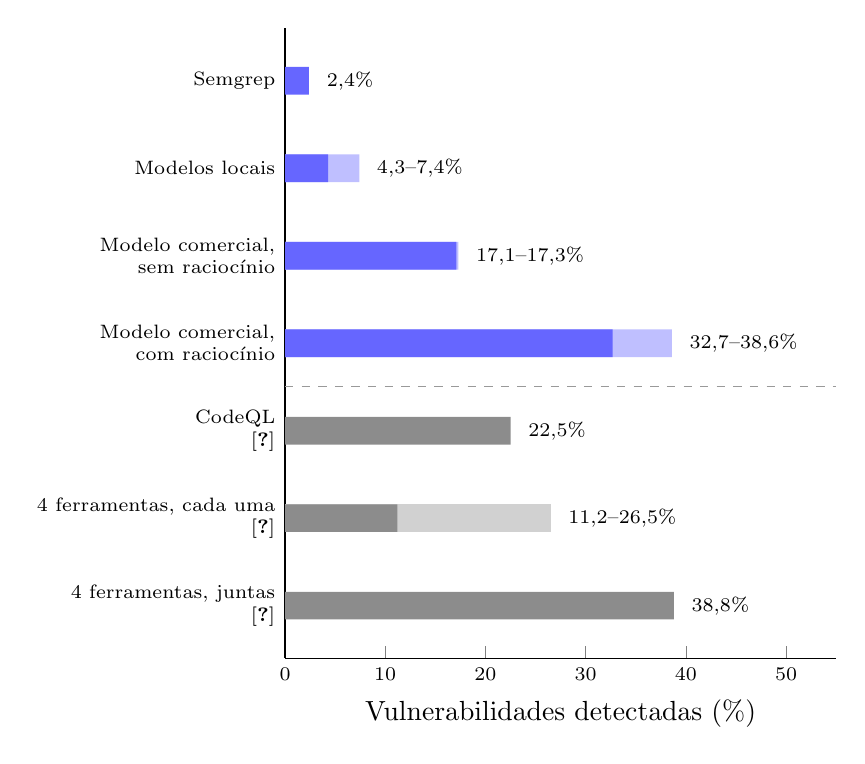
\begin{tikzpicture}
        \begin{axis}[
            scale only axis,
            width=7cm, height=8cm,
            xmin=0, xmax=55, ymin=0.4, ymax=7.6,
            xtick={0,10,...,50},
            ytick={1,2,3,4,5,6,7},
            yticklabels={
                {Semgrep},
                {Modelos locais},
                {Modelo comercial,\\sem raciocínio},
                {Modelo comercial,\\com raciocínio},
                {CodeQL\\\cite{li2025iris}},
                {4 ferramentas, cada uma\\\cite{bennett2024semgrep}},
                {4 ferramentas, juntas\\\cite{bennett2024semgrep}}},
            yticklabel style={align=right},
            tick label style={font=\scriptsize},
            ytick style={draw=none},
            axis x line*=bottom,
            axis y line*=left,
            xlabel={Vulnerabilidades detectadas (\%)},
            y dir=reverse,
            clip=false,
            every axis plot/.append style={xbar, bar width=10pt, bar shift=0pt, draw=none},
        ]
            % Este trabalho, em Go: trecho claro até o maior valor, escuro até o menor
            \addplot[fill=blue!25] coordinates {(7.41,2) (17.3,3) (38.6,4)};
            \addplot[fill=blue!60] coordinates {(2.38,1) (4.31,2) (17.1,3) (32.7,4)};
            % Estudos sobre Java
            \addplot[fill=black!18] coordinates {(26.5,6)};
            \addplot[fill=black!45] coordinates {(22.5,5) (11.2,6) (38.8,7)};
            % Separação entre os dois grupos
            \draw[dashed, black!40] (axis cs:0,4.5) -- (axis cs:55,4.5);
            % Valores
            \node[font=\scriptsize, anchor=west] at (axis cs:3.2,1) {2,4\%};
            \node[font=\scriptsize, anchor=west] at (axis cs:8.2,2) {4,3--7,4\%};
            \node[font=\scriptsize, anchor=west] at (axis cs:18.1,3) {17,1--17,3\%};
            \node[font=\scriptsize, anchor=west] at (axis cs:39.4,4) {32,7--38,6\%};
            \node[font=\scriptsize, anchor=west] at (axis cs:23.3,5) {22,5\%};
            \node[font=\scriptsize, anchor=west] at (axis cs:27.3,6) {11,2--26,5\%};
            \node[font=\scriptsize, anchor=west] at (axis cs:39.6,7) {38,8\%};
        \end{axis}
    \end{tikzpicture}
    \fontepesquisa
\end{figure}

\subsubsection{Diferenças Adicionais}

Além da unidade de rotulagem, outras quatro diferenças ajudam a explicar a distância. A primeira é a \textbf{linguagem}, pois os trabalhos citados avaliam Java, enquanto este avalia Go, cujo ferramental de análise estática ainda é menos maduro. Apenas 84 das 1.074 regras do \texttt{p/default} se aplicam a Go, e a edição comunitária do SonarQube não traz nenhuma regra de segurança para a linguagem. A segunda é a \textbf{natureza dos dados}, porque o F1 de 0,912 do \textit{ZeroFalse} foi medido sobre o \textit{OWASP Benchmark}, um conjunto de código sintético escrito para testar ferramentas, ao passo que a base deste trabalho é toda de código real. O conjunto de código real usado por eles, o \textit{OpenVuln}, reúne apenas 58 alertas.

A terceira diferença é o \textbf{insumo fornecido ao modelo}, já que o \textit{ZeroFalse} entrega ao modelo o caminho completo do dado, da origem até a função crítica, e neste trabalho nenhum dos alertas verificados trouxe esse caminho (Seção~\ref{subsec:q3secas}). A quarta está no \textbf{tamanho dos modelos}, porque o \textit{ZeroFalse} trabalha com modelos de topo de linha e este trabalho, com modelos locais quantizados, de 7 e 9 bilhões de parâmetros, e com um modelo comercial de faixa econômica, com e sem raciocínio.

Por fim, é preciso cuidado ao comparar o F1, porque ele muda muito conforme a proporção de vulneráveis no conjunto. No modo de filtro, em que o modelo recebe só os alertas do Semgrep e decide quais manter, apenas 19 dos 827 alertas são vulneráveis, ou 2,3\%. O especialista do \texttt{qwen2.5-coder:7b} na Rodada 3, por exemplo, manteve 15 alertas, dos quais 3 eram vulneráveis, uma precisão de 20\%. O número parece baixo, mas a proporção de vulneráveis entre os alertas mantidos é quase nove vezes maior que na pilha original. É por isso que a metodologia inclui o MCC, que leva esse desbalanceamento em conta (Seção~\ref{sec:metricas}).

\subsection{O Padrão de Supressão Excessiva}
\label{subsec:supressao}

Como mostrado na Seção~\ref{sec:geral}, a TRA sozinha engana, porque um classificador que descartasse todos os alertas teria a TRA máxima. A Figura~\ref{fig:tra-tfn} coloca as configurações do \texttt{qwen2.5-coder:7b} no plano formado pela TRA e pela TFN, junto desse classificador, que responde ``não é vulnerabilidade'' para tudo e fica no canto superior direito.

\begin{figure}[htpb]
    \centering
    \caption[O compromisso entre TRA e TFN]{Redução de alertas e falsos negativos sobre a pilha de alertas do \texttt{qwen2.5-coder:7b}. Os pontos da Rodada 3 são do modo de filtro, e os das Rodadas 4 e 5 são da pilha lida no modo de triagem. O canto superior direito é o classificador que descarta todos os alertas. TFN calculada sobre os 19 casos vulneráveis}
    \label{fig:tra-tfn}
    \begin{tikzpicture}
        \begin{axis}[
            xmin=0.80, xmax=1.02, ymin=0.40, ymax=1.06,
            width=0.8\textwidth, height=7.5cm,
            xlabel={Taxa de Redução de Alertas (TRA)},
            ylabel={Taxa de Falsos Negativos (TFN)},
            xtick={0.80,0.85,0.90,0.95,1.00},
            ytick={0.4,0.6,0.8,1.0},
            xticklabel style={/pgf/number format/.cd, fixed, fixed zerofill, precision=2, use comma},
            yticklabel style={/pgf/number format/.cd, fixed, fixed zerofill, precision=1, use comma},
            tick label style={font=\scriptsize},
            label style={font=\footnotesize},
        ]
            \addplot[dashed, red!70, thick] coordinates {(0.80,1.0) (1.0,1.0) (1.0,0.40)};
            % O quadrado vem antes, para que o ponto da Rodada 4 fique visível por cima
            \addplot[only marks, mark=square*, mark size=3pt, red!70] coordinates {(1.0,1.0)};
            \addplot[only marks, mark=*, mark size=2.5pt, blue!70] coordinates {
                (0.8497,0.5789) (0.9819,0.8421) (0.9504,0.6842) (0.9976,1.0)};
            \node[font=\scriptsize, anchor=west] at (axis cs:0.853,0.5789) {\textit{baseline} (R3)};
            \node[font=\scriptsize, anchor=east] at (axis cs:0.978,0.8421) {especialista (R3)};
            \node[font=\scriptsize, anchor=east] at (axis cs:0.946,0.6842) {especialista direto (R5)};
            \node[font=\scriptsize, anchor=east, align=right] (r4) at (axis cs:0.972,0.935) {\textit{baseline} sem campos\\do alerta (R4)};
            \draw[-{Latex[length=1.5mm]}, black!60] (r4.east) -- (axis cs:0.9955,0.993);
            \node[font=\scriptsize, text=red!70, anchor=south east] at (axis cs:1.0,1.01) {classificador que descarta tudo};
        \end{axis}
    \end{tikzpicture}
    \fontepesquisa
\end{figure}

O especialista da Rodada 3 descarta 98,2\% dos alertas, mas deixa passar 84,2\% dos vulneráveis, e por isso fica mais perto do canto que descarta tudo do que do \textit{baseline}. É o que este trabalho chama de \textbf{supressão excessiva}: o modelo reduz a pilha descartando quase tudo, inclusive o que é vulnerável. O caso extremo é o \textit{baseline} sem os campos do alerta, na Rodada 4, que descarta 822 dos 824 alertas, entre eles todos os 19 vulneráveis. A TRA dele é a mais alta do experimento, mas não indica ganho nenhum. Sem a mensagem do Semgrep, o modelo simplesmente responde ``não'' para quase tudo, e esse é o exemplo mais claro de por que a TRA só pode ser lida junto da TFN.

O especialista direto da Rodada 5 fica mais longe do canto, porque deixa passar menos vulneráveis, mas em troca mantém mais alertas na pilha. A auditoria da Seção~\ref{sec:q4} confirma o padrão pelo lado qualitativo. Na maior parte dos descartes auditados, a justificativa do modelo não analisa o caso e apenas repete uma disposição geral a descartar.

A sétima rodada (Seção~\ref{subsec:q1fichas}) ajuda a entender por que isso acontece. O \textit{baseline} e o especialista julgam exatamente o mesmo código, e o especialista recebe a mais só uma orientação sobre o tipo de fraqueza. Se o modelo usasse essa orientação para entender melhor o código, ele reconheceria mais vulneráveis e daria menos alarmes falsos ao mesmo tempo. Nos modelos locais, isso não aconteceu em nenhuma configuração, e o que a orientação fez foi deslocar o \textbf{limiar de decisão}, isto é, a facilidade com que o modelo responde ``vulnerável''.

Com o \texttt{qwen2.5-coder:7b}, as fichas por CWE, que sempre terminam com um critério de descarte e trazem um exemplo inofensivo, empurraram o modelo para o ceticismo. Ele passou de 8 para 3 vulneráveis reconhecidos e de 116 para 12 alarmes falsos (Tabela~\ref{tab:filtro}). Com as fichas por regra, voltou a alarmar mais, sem reconhecer mais vulneráveis. Com o \texttt{gemma2:9b}, o deslocamento foi para o lado oposto, porque a ficha da CWE-327, que trata de \textit{hash} fraco, se misturou com a mensagem do alerta, que trata de TLS, e gerou 57 alarmes falsos que desapareceram com a ficha por regra.

O que os dois modelos têm em comum, portanto, não é a direção do erro, e sim a causa. O modelo local alarma quando o \textit{prompt} descreve um perigo parecido com algo que ele vê no código ou no alerta, e descarta quando o \textit{prompt} o orienta a descartar. Ele repete a descrição do perigo em vez de aplicar a condição que vem junto, o mesmo padrão que a auditoria da Seção~\ref{sec:q4} encontrou com a mensagem do alerta. Nos modelos locais avaliados, a orientação muda a postura do modelo, mas não aprofunda a análise do código.

Esse padrão não é exclusivo de modelos pequenos. No conjunto real do \textit{ZeroFalse}, o \textit{gemini-2.5-pro}, um modelo de topo de linha, tem precisão perfeita, mas \textit{recall} de apenas 0,229 e F1 de 0,372, o pior resultado daquele conjunto. Os autores atribuem esse comportamento a ``estratégias de supressão excessivamente conservadoras'', que não se sustentam em dados reais ruidosos \cite{iranmanesh2025zerofalseimprovingprecisionstatic}.

A supressão excessiva, contudo, não é inevitável, e o modelo comercial avaliado aqui não a apresenta. No modo de filtro, ele descarta de 66\% a 70\% dos alertas e deixa passar de 37\% a 53\% dos vulneráveis, e ficaria fora da Figura~\ref{fig:tra-tfn}, à esquerda, porque o erro dele é o contrário, o excesso de alarmes (Seção~\ref{sec:modelos}). Mesmo assim, o mecanismo é o mesmo, já que a orientação do \textit{prompt} deslocou o limiar dele na direção do alarme, como no \texttt{gemma2:9b}, e de novo com os alarmes concentrados na CWE-327. O raciocínio reforça essa leitura, pois, ligado, empurrou o modelo comercial ainda mais para o alarme no modo de triagem, com os dois \textit{prompts}, e só com o especialista esse deslocamento veio acompanhado de melhor discriminação (Seção~\ref{sec:modelos}). A supressão é, assim, só uma das posições a que esse deslocamento pode levar, e quem decide qual delas é o modelo e a orientação.

\subsection{Comparação com Abordagens de Eliminação Sã}
\label{subsec:saeliminacao}

Um método de eliminação de alarmes é chamado de \textbf{são} quando garante que nunca descarta um alarme verdadeiro. A filtragem por modelo de linguagem não tem essa garantia, e a taxa de falsos negativos medida aqui mostra o custo disso.

Um exemplo de abordagem sã é o \textit{Rican} \cite{wang2026rican}, que elimina alarmes executando o programa. Ele se aplica aos alarmes em que o defeito acontece ou não do mesmo jeito em cada caminho do programa, qualquer que seja a entrada, propriedade que os autores chamam de \textit{input-agnosticity}. Nesses casos, basta executar uma vez cada caminho até o ponto do alarme, e, se o defeito não aparece, o alarme é falso com garantia. Sobre 2.912 alarmes em seis projetos reais, o método elimina 1.313 (45,09\%) \textbf{sem eliminar nenhum alarme verdadeiro}.

O contraste deixa claro o compromisso entre as duas abordagens. A abordagem sã remove menos alertas, mas não perde nenhuma vulnerabilidade. Já a filtragem com o especialista do \texttt{qwen2.5-coder:7b} remove 98,19\% dos alertas, mas deixa passar 16 dos 19 vulneráveis que chegam a ela. São dois pontos de um mesmo espaço de decisão, e a escolha entre eles depende do que custa mais caro, revisar um alarme falso ou deixar escapar uma vulnerabilidade. Os números não servem para dizer qual abordagem é melhor, porque as linguagens, os analisadores e os dados são diferentes, e a comparação serve apenas para mostrar que cada uma faz uma escolha diferente entre remover alertas e não perder vulnerabilidades.

\subsection{Consequências para a Arquitetura Híbrida}
\label{subsec:consequencias}

A expectativa corrente na literatura é que o componente neural compense os pontos cegos do componente simbólico \cite{li2025iris}, isto é, que o modelo encontre o que o analisador deixa passar. Os resultados deste trabalho não sustentam essa expectativa na configuração avaliada, porque os casos que o analisador perde também são, na maior parte, perdidos pelo modelo. Dos 778 casos que o Semgrep não detecta, os modelos locais reconhecem 4,31\% e 7,41\% com o especialista direto, e a única forma de aumentar esse número foi fazer o modelo responder ``vulnerável'' com mais frequência, o que encheu a pilha de alarmes falsos.

O modelo comercial vai mais longe, pois sem raciocínio reconhece de 17,1\% a 17,3\% desses casos sem precisar desse deslocamento e, com raciocínio, chega a 32,7\% no esforço baixo e a 38,6\% no alto. Só o primeiro aumento, porém, veio com ganho real de discriminação. No esforço alto, o modelo passou a alarmar mais também nos seguros, sem separar melhor o vulnerável do seguro, e mesmo no melhor caso deixa de fora 61,4\% desses casos.

O que a arquitetura entrega, portanto, é redução de ruído sobre aquilo que o analisador já encontra. Com o \texttt{qwen2.5-coder:7b} e o especialista, essa redução é robusta, repetida em três populações, e vem com discriminação modesta, mas positiva (MCC de $+0{,}161$), embora ao custo de perder a maior parte dos vulneráveis da pilha. Ela também depende do modelo, já que nem o \texttt{gemma2:9b} nem o modelo comercial reproduzem, no modo de filtro, o ganho do especialista, e o comercial remove menos ruído que o \texttt{qwen2.5-coder:7b}. Essas são as duas conclusões centrais do trabalho. O modelo não recupera o que o analisador perde, mas reduz o ruído daquilo que o analisador encontra.

Os resultados sugerem que o modelo de linguagem seria mais útil antes do analisador, e não depois. A Seção~\ref{subsec:sobra} mostrou que parte das vulnerabilidades escapa porque a operação perigosa fica atrás de funções do próprio projeto, que as regras do Semgrep não reconhecem.

O \textit{MEMHINT} \cite{huang2026memhint} enfrentou um problema parecido em C/C++, com vazamentos de memória escondidos em funções do próprio projeto. Ele usa um modelo de linguagem para identificar essas funções, confere a classificação de forma simbólica e passa o resultado ao analisador, e com isso detectou 54 vazamentos, contra 19 do CodeQL e 2 do Semgrep. O \textit{IRIS} \cite{li2025iris} faz o mesmo para a análise de fluxo de dados em Java.

Neste trabalho, a mesma estratégia consistiria em usar o modelo de linguagem para identificar, em cada projeto, as funções que recebem entrada externa, as que manipulam caminhos de arquivo e as que sanitizam dados, e converter essa classificação em regras do Semgrep. Entre elas estariam as funções de bibliotecas como a \texttt{afero}, que troca as funções de arquivo da biblioteca padrão por outras e, assim, esconde a operação perigosa das regras atuais (Figura~\ref{fig:abstracao}), e os campos de \textit{struct} que recebem entrada externa.

Nessa posição, antes do analisador, o modelo poderia de fato aumentar a detecção, o que não acontece quando ele só filtra os alertas depois. A abordagem também evita o risco discutido na Seção~\ref{subsec:h4}, de as regras descreverem só os casos usados para escrevê-las, porque aqui ninguém escreve regras olhando os casos. O modelo classifica as funções de cada projeto, e uma verificação simbólica confere essa classificação antes de ela virar regra.

Mesmo assim, a estratégia não resolveria tudo. Em 25,4\% dos casos de CWE-22 e 48,2\% dos de CWE-918, a operação perigosa nem está no arquivo rotulado como vulnerável (Seção~\ref{subsec:sobra}), e nenhuma regra consegue encontrar num arquivo algo que não está nele. É uma direção para trabalho futuro, que este trabalho não chegou a testar.
